%%%%%%%% ICML 2023 EXAMPLE LATEX SUBMISSION FILE %%%%%%%%%%%%%%%%%

\documentclass{article}

% Recommended, but optional, packages for figures and better typesetting:
\usepackage{microtype}
\usepackage{graphicx}
\usepackage{subfigure}
\usepackage{booktabs} % for professional tables

% hyperref makes hyperlinks in the resulting PDF.
% If your build breaks (sometimes temporarily if a hyperlink spans a page)
% please comment out the following usepackage line and replace
% \usepackage{icml2023} with \usepackage[nohyperref]{icml2023} above.
\usepackage{hyperref}


\newcommand{\arash}[1]{\textcolor{red}{[AV: #1]}}
\newcommand{\weili}[1]{\textcolor{blue}{[WN: #1]}}

% Attempt to make hyperref and algorithmic work together better:
\newcommand{\theHalgorithm}{\arabic{algorithm}}

% Use the following line for the initial blind version submitted for review:
% \usepackage{icml2023}

% If accepted, instead use the following line for the camera-ready submission:
\usepackage[accepted]{icml2023}
% \usepackage[preprint]{icml2023}

% For theorems and such
\usepackage{amsmath}
\usepackage{amssymb}
\usepackage{mathtools}
\usepackage{amsthm}
\usepackage{enumitem}
% if you use cleveref..
\usepackage[capitalize,noabbrev]{cleveref}

%%%%%%%%%%%%%%%%%%%%%%%%%%%%%%%%
% THEOREMS
%%%%%%%%%%%%%%%%%%%%%%%%%%%%%%%%
\theoremstyle{plain}
\newtheorem{theorem}{Theorem}[section]
\newtheorem{proposition}[theorem]{Proposition}
\newtheorem{lemma}[theorem]{Lemma}
\newtheorem{corollary}[theorem]{Corollary}
\theoremstyle{definition}
\newtheorem{definition}[theorem]{Definition}
\newtheorem{assumption}[theorem]{Assumption}
\theoremstyle{remark}
\newtheorem{remark}[theorem]{Remark}

% Todonotes is useful during development; simply uncomment the next line
%    and comment out the line below the next line to turn off comments
%\usepackage[disable,textsize=tiny]{todonotes}
\usepackage[textsize=tiny]{todonotes}

\input{math_commands.tex}
\newcommand{\df}{\mathrm{d}}
\newcommand{\din}{d_{\mathrm{in}}}
\newcommand{\dout}{d_{\mathrm{out}}}
\theoremstyle{plain}
% \newtheorem{theorem}{Theorem}[section]
% \newtheorem{proposition}[theorem]{Proposition}
% \newtheorem{lemma}[theorem]{Lemma}
% \newtheorem{corollary}[theorem]{Corollary}
% \theoremstyle{definition}
% \newtheorem{definition}[theorem]{Definition}
% \newtheorem{assumption}[theorem]{Assumption}
% \theoremstyle{remark}
% \newtheorem{remark}[theorem]{Remark}

% The \icmltitle you define below is probably too long as a header.
% Therefore, a short form for the running title is supplied here:
\icmltitlerunning{Fast Sampling of Diffusion Models via Operator Learning}

\begin{document}

\twocolumn[
\icmltitle{Fast Sampling of Diffusion Models via Operator Learning}

% It is OKAY to include author information, even for blind
% submissions: the style file will automatically remove it for you
% unless you've provided the [accepted] option to the icml2023
% package.

% List of affiliations: The first argument should be a (short)
% identifier you will use later to specify author affiliations
% Academic affiliations should list Department, University, City, Region, Country
% Industry affiliations should list Company, City, Region, Country

% You can specify symbols, otherwise they are numbered in order.
% Ideally, you should not use this facility. Affiliations will be numbered
% in order of appearance and this is the preferred way.
% \icmlsetsymbol{equal}{*}

\begin{icmlauthorlist}
\icmlauthor{Hongkai Zheng}{yyy}
\icmlauthor{Weilie Nie}{comp}
\icmlauthor{Arash Vahdat}{comp}
\icmlauthor{Kamyar Azizzadenesheli}{comp}
\icmlauthor{Anima Anandkumar}{yyy,comp}
% \icmlauthor{Firstname6 Lastname6}{sch,yyy,comp}
% \icmlauthor{Firstname7 Lastname7}{comp}
%\icmlauthor{}{sch}
% \icmlauthor{Firstname8 Lastname8}{sch}
% \icmlauthor{Firstname8 Lastname8}{yyy,comp}
%\icmlauthor{}{sch}
%\icmlauthor{}{sch}
\end{icmlauthorlist}

\icmlaffiliation{yyy}{Caltech}
\icmlaffiliation{comp}{NVIDIA}
% \icmlaffiliation{sch}{School of ZZZ, Institute of WWW, Location, Country}

\icmlcorrespondingauthor{Hongkai Zheng}{hzzheng@caltech.edu}
% \icmlcorrespondingauthor{Firstname2 Lastname2}{first2.last2@www.uk}

% You may provide any keywords that you
% find helpful for describing your paper; these are used to populate
% the "keywords" metadata in the PDF but will not be shown in the document
\icmlkeywords{Machine Learning, ICML}

\vskip 0.3in
]

% this must go after the closing bracket ] following \twocolumn[ ...

% This command actually creates the footnote in the first column
% listing the affiliations and the copyright notice.
% The command takes one argument, which is text to display at the start of the footnote.
% The \icmlEqualContribution command is a standard text for equal contribution.
% Remove it (just {}) if you do not need this facility.

\printAffiliationsAndNotice{}  % leave blank if no need to mention the equal contribution
% \printAffiliationsAndNotice{\icmlEqualContribution} % otherwise use the standard text.

\begin{abstract}
Diffusion models have found widespread adoption in various areas. However, their sampling process is slow because it requires hundreds to thousands of network evaluations to emulate a continuous process defined by differential equations. In this work, we use neural operators, an efficient method to solve the probability flow differential equations, to accelerate the sampling process of diffusion models. Compared to other fast sampling methods that have a sequential nature, we are the first to propose a parallel decoding method that generates images with only one model forward pass. We propose \textit{diffusion model sampling with neural operator} (DSNO) that maps the initial condition, i.e., Gaussian distribution, to the continuous-time solution trajectory of the reverse diffusion process. To model the temporal correlations along the trajectory, we introduce temporal convolution layers that are parameterized in the Fourier space into the given diffusion model backbone. We show our method achieves state-of-the-art FID of 3.78 for CIFAR-10 and 7.83 for ImageNet-64 in the one-model-evaluation setting. 
% Previously, parallel decoding was only proposed with discrete tokens. 
% Compared to other fast sampling methods that still have a sequential nature, DSNO leverages parallel decoding to predict the solution trajectory and thus is more efficient.
% is built upon the diffusion model architecture and temporal convolution blocks that are parameterized in the Fourier space. 
% Our sampling method can be applied to any existing pre-trained diffusion models and generate high-quality samples in one model forward call. 
% Compared to other fast sampling methods with a sequential nature such as progressive distillation, DSNO uses parallel decoding \footnote{In this paper, the term "parallel decoding" refers to the class of methods that generates the target trajectory in parallel. } to output the continuous-in-time trajectory and thus is efficient in sampling. 
% Compared to other fast sampling methods that have a sequential nature, we are the first to propose a parallel decoding method to generate the trajectory of images in one model evaluation. 
\end{abstract}





\section{Introduction}


\begin{figure*}[t]
        \centering
        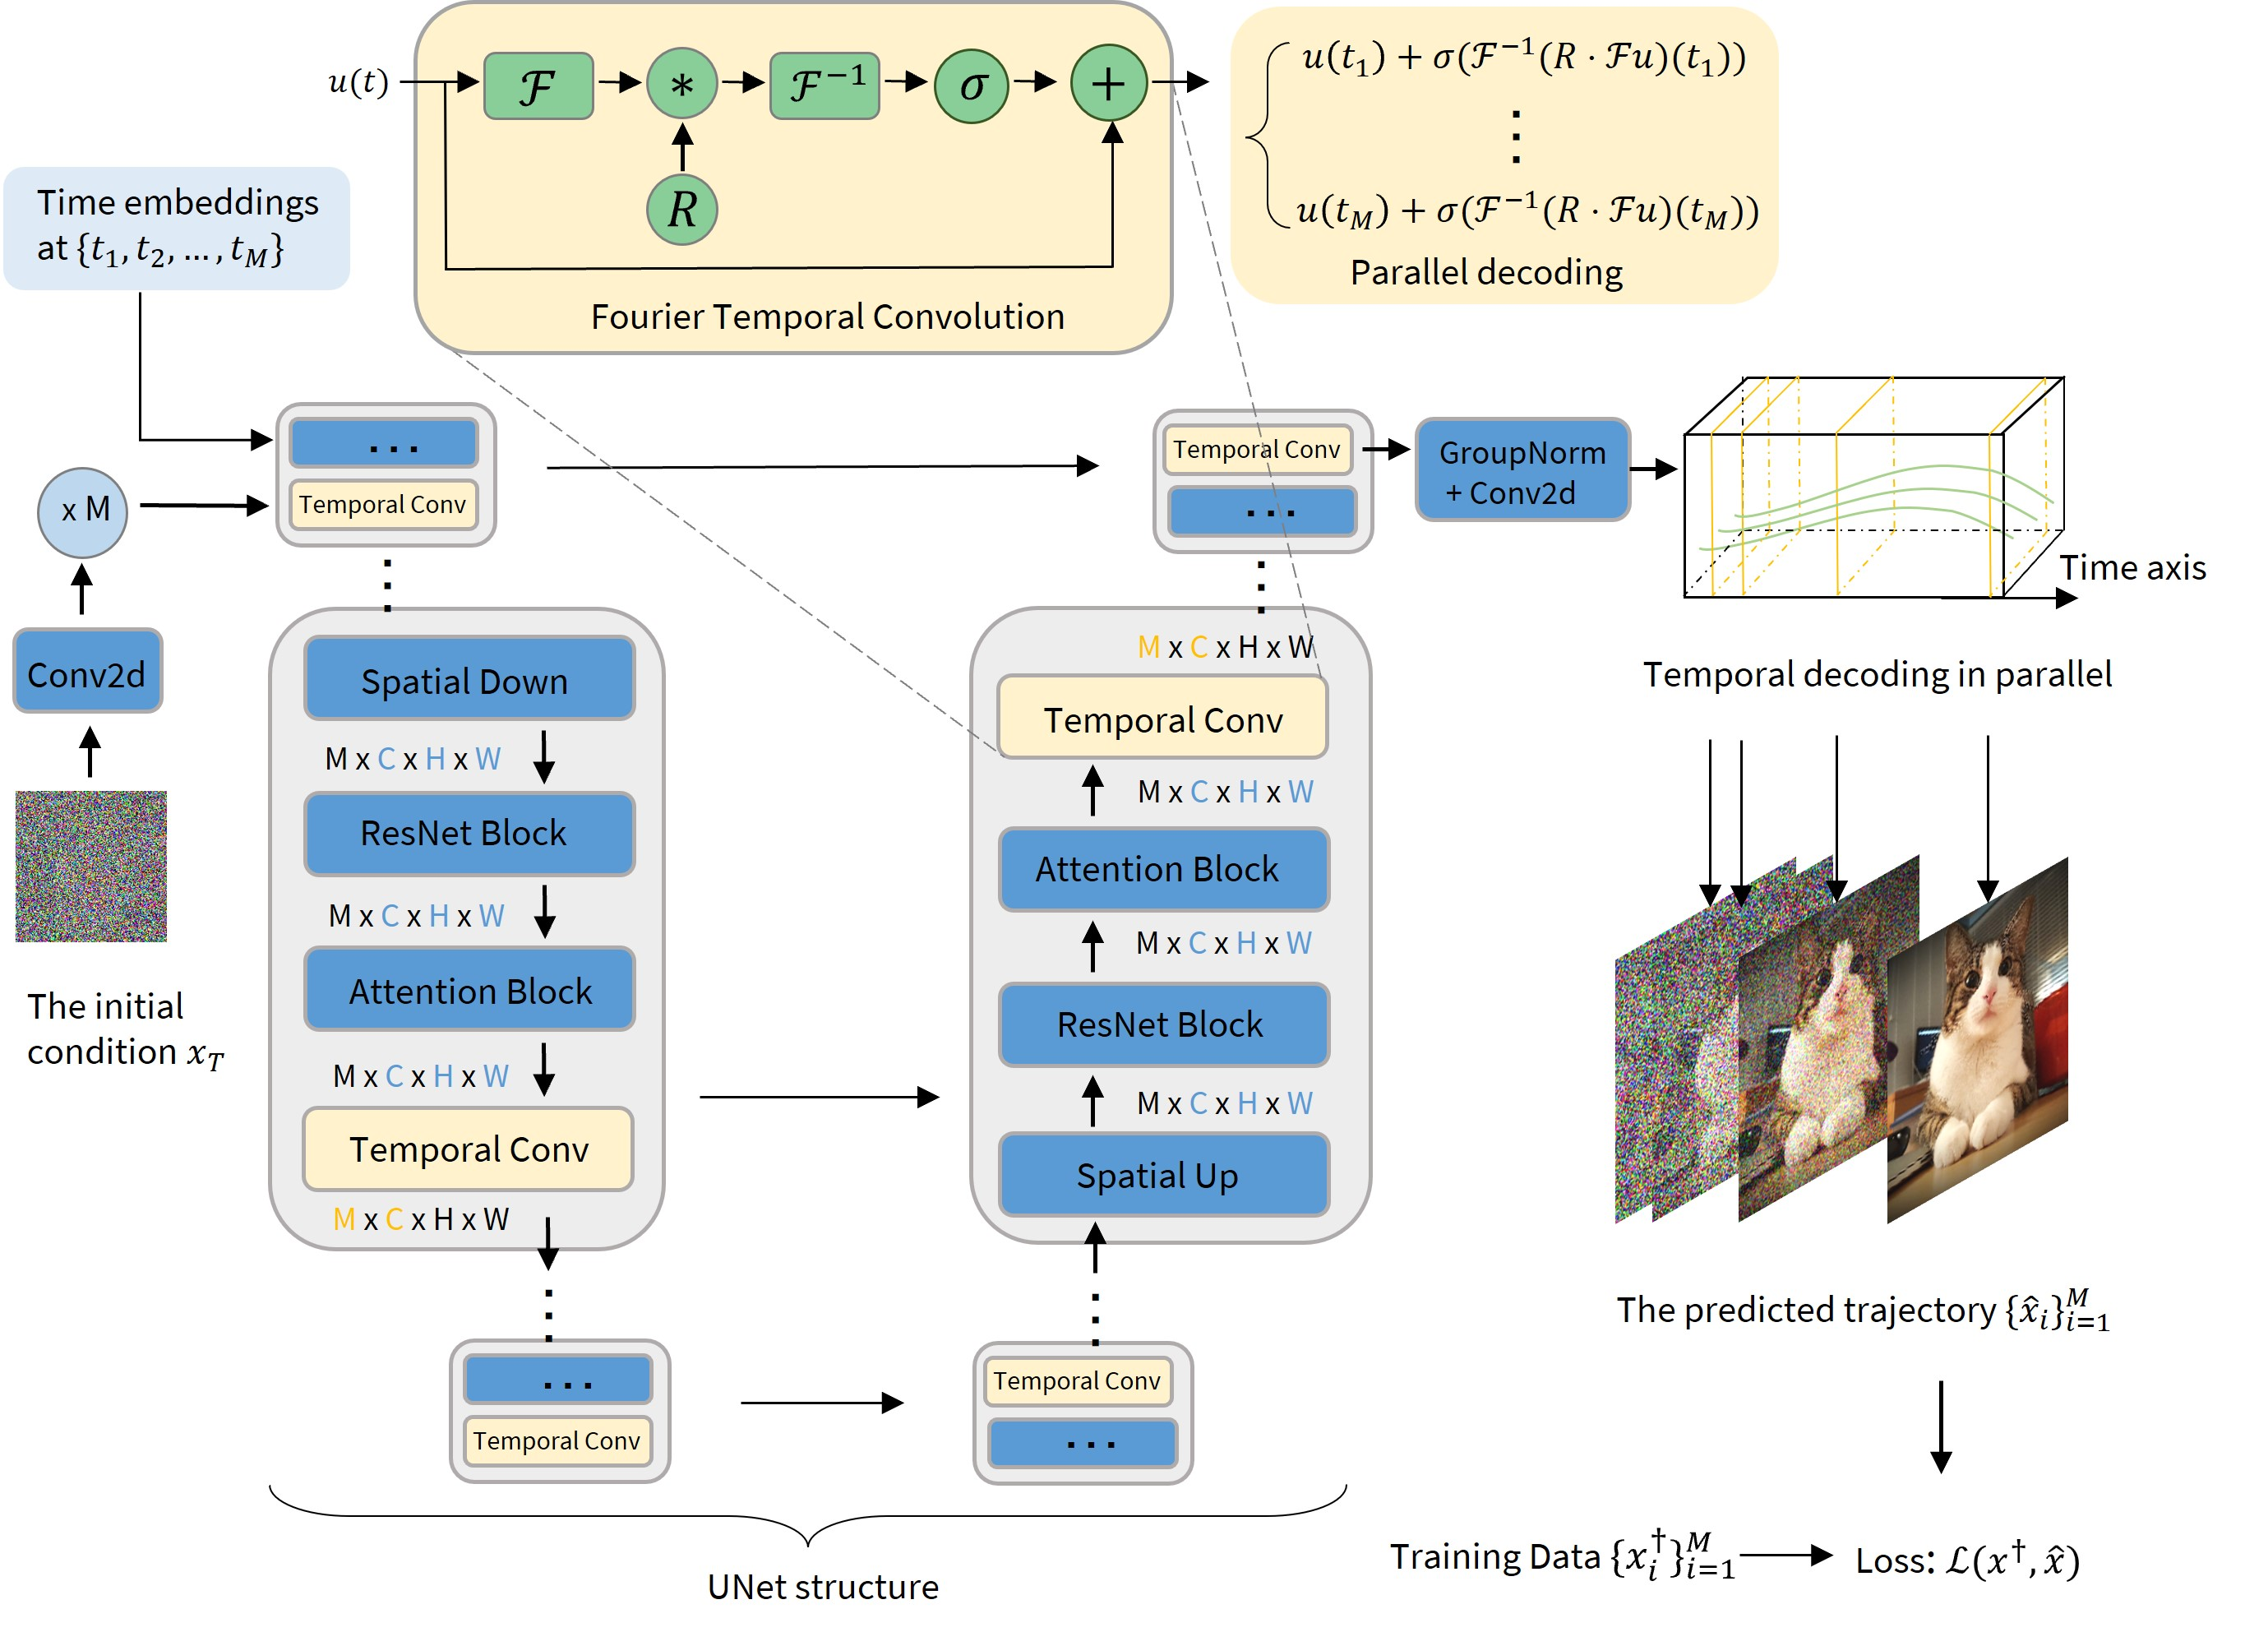
\includegraphics[width=0.92\textwidth]{figs/arch_v3-3.jpg}
        \caption{Illustration of the architecture and training pipeline of DSNO. The architecture of DSNO is built on top of any existing diffusion model architecture, where blue blocks are from the existing diffusion U-Net backbone and yellow blocks are the proposed temporal convolution layers.
        % introduced at each level of the UNet backbone. 
        % As indicated by the highlighted dimensions of the feature map, 
        Suppose the temporal domain is discretized into $M$ points $\{t_1,\dots,t_M\}$,
        % which is not necessarily a uniform grid,
        for each feature map, the temporal convolution layers operate on the temporal and channel dimensions (M$\times$C) and the other blocks operate on the pixel and channel dimensions (C$\times$H$\times$W). The symbols $\gF$ and $\gF^{-1}$ refer to the Fourier transform and inverse Fourier transform, respectively. 
        $R$ is a complex-valued parameter that represents a kernel function in Fourier space. For ease of notation, $x_i$ represents the solution at time $t_i$, that is $x(t_i)$. 
        Inside each temporal convolution layer, we apply the idea of parallel decoding: Given input function $u(t)$, the Fourier coefficients $R\cdot \gF u$ is the same for all $t_i, i=1,\dots, M$. Therefore, the temporal convolution layer can output the representations at different time locations in the trajectory in a single forward pass by evaluating the output function at queried points in parallel.}
        \label{fig:dfno_arch}
\end{figure*}




Diffusion models~\citep{sohl2015deep,ho2020denoising}, also known as score-based generative models~\citep{song2020score}, have emerged as a powerful generative modeling framework in various areas. They have achieved state-of-the-art (SOTA) performance in many applications including image generation \cite{dhariwal2021diffusion}, molecule generation \cite{xu2022geodiff}, audio synthesis \cite{kong2021diffwave} and model robustness~\cite{nie2022DiffPure}. However, sampling from diffusion models requires hundreds of neural network evaluations, making them slower by orders of magnitude compared to other generative models such as generative adversarial networks (GANs) \cite{goodfellow2020generative}. Accelerating sampling in diffusion models remains a challenging but important problem, especially when applying them to time-sensitive downstream applications such as AI for art and design \cite{ramesh2022hierarchical} or generative models for decision making \cite{ajay2022conditional}. 

Existing methods for fast sampling of diffusion models can be summarized into two main categories: 1) \emph{training-free sampling methods}~\citep{song2020denoising,lu2022dpm} and 2) \emph{training-based sampling methods}~\citep{luhman2021knowledge,salimans2021progressive,xiao2021tackling}. Specifically, the training-free methods focus on reducing the number of discretization steps from a numerical perspective while solving the stochastic differential equations (SDE) or probability flow ordinary differential equations (ODE). However, even the best well-designed numerical solvers \cite{lu2022dpm, karras2022elucidating} still need 10$\sim$30 model evaluations such that the approximation error is small enough for an acceptable sampling quality.
% generating reasonable-quality samples, which is still a big gap from real-time sampling. 
On the other hand, training-based methods train a  surrogate network to replace some parts of the numerical solver or even the whole solver. Particularly, progressive distillation \cite{salimans2021progressive} has made a big step towards real-time sampling (e.g., decent results with 4 steps) but it still has a sequential nature like conventional numerical solvers. %and comes at the price of a high training cost. 

 % Most prior works including training-based methods follow the structure of numerical solvers and solve the equation step by step. 
The goal of this work is to develop a fast and parallel sampling method for diffusion models \emph{with only one model evaluation}. By parallel, we mean that our method can decode images at different time locations in the trajectory in parallel and hence, generate the final solution using only one model evaluation. The major challenge here arises from the difficulty of solving a complicated and large-scale differential equation, which typically requires many discrete time steps to emulate accurately from a numerical approximation perspective. 

% On the contrary, the recent advancements in operator learning for solving differential equations open new doors to solving differential equations. 
In this paper, we employ the recent advances in neural operators for solving differential equations to overcome this challenge. 
Neural operators \citep{li2020neural,kovachki2021neural}, especially the Fourier neural operator (FNO)~\cite{li2020fourier} have shown several orders of magnitude speedup over conventional solvers. This class of models enables learning maps between spaces of functions and is shown to be discretization invariant, allowing them to work with different resolutions of data without changing the model parameters, and can approximate any given nonlinear continuous operator~\cite{kovachki2021universal}. 

%Therefore, two natural questions arise: is
The FNO allows for parallel decoding: i.e. the outputs at all locations of the trajectory can be simultaneously evaluated. This is a property that none of the previous sampling methods for diffusion models enjoy.   
% The success of neural operators in other scientific applications raises the question that whether it is possible to design a neural operator to accelerate the sampling process of diffusion models and if yes how.
In this work, we propose a neural operator for diffusion model sampling (DSNO) that maps the initial conditions (i.e. Gaussian distribution) to the solution trajectories and we show its effectiveness in both unconditional and class-conditional image generation. 


% and directly acquiring the continuous-in-time dynamics of the underlying diffusion model.

% \paragraph{Training-free sampling methods} focus on solving the reverse stochastic differential equation (SDE) or the corresponding probability flow ordinary differential equation (ODE) from a numerical perspective. SDE-based samplers~\cite{karras2022elucidating, song2020score} often have better sample quality than ODE-based samplers but they are much slower. They typically require hundreds if not thousands of score model evaluations because they use small time steps to emulate the continuous-time stochastic process. ODE-based methods \cite{song2021denoising, lu2022dpm, zhang2022fast} are built upon the deterministic reverse process. It allows the solver to take larger time steps while keeping the approximation error small but they still need more than 10 score model evaluations to generate high-quality samples.  
% % by leveraging some special structures of the underlying ODE such as semi-linear structure and the form of exponentially weighted integral \cite{lu2022dpm, zhang2022fast}. Existing works \cite{song2021denoising, bao2021analytic, zhang2022fast} have greatly reduced the number of discretization steps in time while keeping the approximation error small but still need more than 10 score model evaluations to generate high-quality samples. 
%  % However, it requires progressive training from fine resolution to coarse resolution. 

% \paragraph{Training-based sampling methods} typically train a neural network surrogate to replace some parts of the numerical solver or even the whole solver. This category includes various methods from diverse perspectives such as knowledge distillation \cite{luhman2021knowledge, salimans2021progressive}, learning the noise schedule \cite{lam2021bilateral, watson2021learning}, learning the reverse covariance \cite{bao2022estimating}, which require extra training. Training-based methods usually work in the few-step regime with less than 10 steps. Direct \citet{luhman2021knowledge} is the first work to get descent sample quality on CIFAR10 with one model evaluation but it suffers from overfitting and its sampling quality drops dramatically compared to the original numerical sampling methods in diffusion models. The current SOTA progressive distillation \cite{salimans2021progressive} reduces the number of steps down to 4-8 without losing much sample quality. However, it breaks in the limit of one function evaluation. 


% The research challenge that we aims to tackle is how to achieve real-time sampling of the existing diffusion models. We have witnessed great advancements in training-free methods but we also see the best well-designed solvers \cite{lu2022dpm, karras2022elucidating} have to take around 10-30 model evaluations such that the approximation error is small enough for generating reasonable-quality samples, which is still a big gap from real-time sampling. On the other hand, the training-based progressive distillation \cite{salimans2021progressive} has made a big step towards the real-time sampling of diffusion models but it still has a sequential nature and comes at the price of a high training cost. The goal of this work is to develop a real-time sampling method that is faster than existing methods by leveraging parallel decoding and directly acquiring the continuous-in-time dynamics of the underlying diffusion model.

% Neural operator \citep{li2020neural,kovachki2021universal} is one of the state-of-the-art machine learning frameworks for solving PDEs. It is a new class of machine learning models designed for mapping between spaces of functions, whose discretization invariant property allows it to work with different resolutions of data without changing the model parameters. Neural operators, especially the Fourier neural operators (FNO)~\cite{li2020fourier}, have shown several orders of magnitude speedup over conventional PDE solvers in many scientific problems. 

% Neural operators are deep learning models that are designed for mappings between function spaces, i.e., continuous functions~\citep{li2020neural,kovachki2021universal}. They are widely deployed as the de facto deep learning models in scientific computing when dealing with partial differential equations (PDE). This class of models enables learning maps between spaces of functions, whose discretization invariant property allows it to work with different resolutions of data without changing the model parameters. Neural operators, especially the Fourier neural operators (FNO)~\cite{li2020fourier}, have shown several orders of magnitude speedup over conventional PDE solvers in many scientific problems~\citep{wen2022accelerating,pathak2022fourcastnet}.


% with temporal convolution blocks parameterized in the Fourier space 
% by leveraging parallel decoding that directly predicts the whole ODE trajectory of diffusion models. 
 \paragraph{Our contributions.}
\begin{itemize}[leftmargin=*]
    % \item We observe that the trajectories of the reverse process of existing pre-trained diffusion models have a compact spectrum. 
    \item We propose a neural operator for the fast sampling of diffusion models (DSNO) that can sample high-quality images with one model evaluation. 
    \item We introduce temporal convolution blocks parameterized in Fourier space, which can be easily combined with any existing neural architectures of diffusion models to build a neural operator backbone for DSNO. Furthermore, our proposed temporal convolution blocks are lightweight and only increase the model size by 10\%.
    \item For the first time, we propose a parallel decoding method to generate the trajectories of images using continuous function representation, which enables generation of the final solution in one model evaluation.
    % \arash{do we need to mention MUSE here? I think their parallel decoding is in the spatial domain, while ours is in the time axis} 
    \item Our proposed DSNO achieves new state-of-the-art FID scores of 3.78 for CIFAR-10 and 7.83 for ImageNet-64 in the setting of single-step-generation of diffusion models.
    % DSNO is efficient in sampling by leveraging parallel decoding compared to other fast sampling methods such as progressive distillation.
    % The sampling speed of the DSNO is 1.3 to 2.6 times faster than the progressive distillation with a better or comparable FID score. 
    % \item DSNO only takes one function evaluation to sample and has better generalization ability than distillation methods. With the trajectory information guiding the sampling, DSNO achieves the state-of-the-art FID of 4.12 for CIFAR-10 and [placeholder] for the ImageNet-64 model
\end{itemize}
% We note that a critical difference between DSNO and the other methods is that DSNO outputs a continuous function so that it can generate the solution trajectory by evaluating the function at different time steps in parallel. In contrast, the other methods have a sequential nature and predict the trajectory step by step. We argue that DSNO with a parallel decoding nature is a key step that can pave the way for the real-time sampling of diffusion models, potentially benefiting many time-sensitive applications of diffusion models. 

Finally, we note that DSNO leverages parallel decoding temporally to generate the solution trajectory by evaluating the output function at different time steps in parallel. This is in contrast to the prior training-based methods that have a sequential nature and predict the trajectory step by step.  %  and can be conditioned on any value of arbitrary time step
We believe that DSNO with parallel decoding is a key step for the real-time sampling of diffusion models, potentially benefiting many interactive applications. 
% We note that the temporally continuous output of DSNO provides another level of flexibility compared to distillation-based methods, and is readily available for applications such as DiffPure~\cite{nie2022DiffPure} that requires fast forward/backward sampling from diffusion models at various temporal locations. 
% \arash{I think the last sentence could be moved to conclusions. It is too early to say what we don't do.}
% Function space representation of DSNO allows ODE evolution throughout the temporal trajectory,

% \begin{figure}[ht]
%         \centering
%         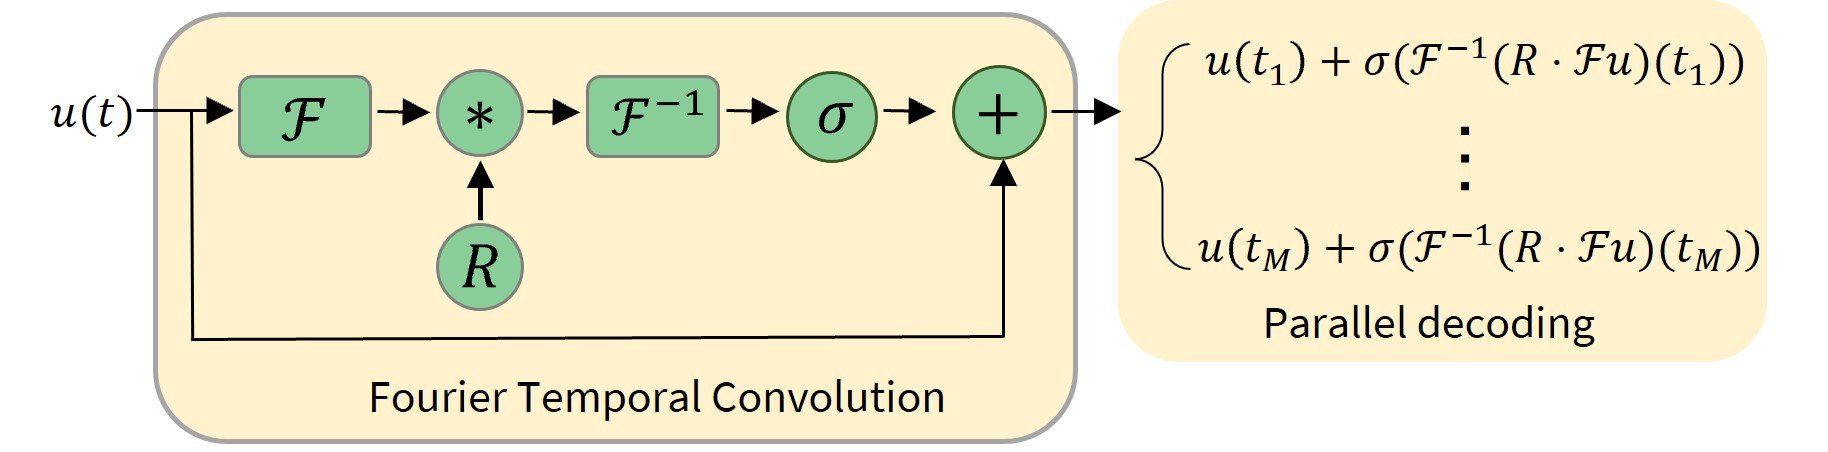
\includegraphics[width=0.98\columnwidth]{figs/parallel_decode.jpg}
%         \caption{Illustration of parallel decoding of the Fourier temporal convolution layer. Given input function $u(t)$, the Fourier coefficients $R\cdot \gF u$ are the same for all $t_i, i=1,\dots, M$. Therefore the temporal convolution layer can output the representations at different times in a single forward pass by evaluating the output function at queried points in parallel. }
%         \label{fig:parallel_decode}
% \end{figure}



\section{Background}
\paragraph{Score-based generative models.} We consider the general class of score-based generative models in a unified continuous-time framework proposed by \citet{song2020score}, which includes different variants of diffusion models \cite{sohl2015deep, ho2020denoising}. In this paper, we will use the word score-based models interchangeably with diffusion models. Suppose the data distribution is $p_{\mathrm{data}}$. The forward pass is a diffusion process $\{\rvx(t)\}$ starting from $0$ to $T$ which can be expressed as
\begin{equation}
    \df \rvx = f(\rvx, t) \df t + g(t) \df \rvw_t,
\end{equation}
where $\rvw_t$ is the standard Wiener process, and $f(\cdot,t): \mathbb{R}^d \rightarrow \mathbb{R}^d$ and $g(\cdot): \mathbb{R}\rightarrow \mathbb{R}$ are the drift and diffusion coefficients respectively. Diffusion models choose $f$ and $g$ such that $\rvx(0)\sim p_{\mathrm{data}}$ and $\rvx(T) \sim \mathcal{N}(0, \textbf{I})$. 
 \citet{song2020score} show that the following probability flow ODE produces the same marginal distributions $p_t(\rvx)$ as that of the diffusion process:
\begin{equation}
    \df \rvx = f(\rvx, t) \df t  - \frac{1}{2}g(t)^2 \nabla_{\rvx}\log p_t(\rvx) \df t.
    \label{eq:prob_ode}
\end{equation}
The sampling process eventually becomes solving the probability flow ODE~\ref{eq:prob_ode} from $T$ to $0$ given the initial condition $\rvx(T)$. Furthermore, $f(\rvx, t)$ often has the affine form $f(\rvx,t) = h(t) \rvx$, where $h: \mathbb{R} \rightarrow \mathbb{R}$. We can simplify the equation~\ref{eq:prob_ode} into a semi-linear ODE. Integrating both sides over time gives the explicit form of solution for any $t<s$:
\begin{equation}
    \rvx(t) = \phi(t, s) \rvx(s) - \int_{s}^{t} \phi(t, \tau) \frac{g(\tau)^2}{2} \nabla_{\rvx}\log p_{\tau}(\rvx) \df \tau, 
    \label{eq:ode_soln}
\end{equation}
where $\phi(t, s) = \exp\left(\int_{s}^{t} h(\tau) \df \tau \right)$. The ODE can be solved using numerical solvers such as Euler's method, multistep methods, and Heun's 2\textsuperscript{nd} method. 
The score function $\nabla_{\rvx} \log p_t(\rvx) $ is usually parameterized by $
    \hat{\epsilon}_{\theta}(\rvx_t) \approx - \sigma_t \nabla_{\rvx} \log p_t(\rvx)$, where $\sigma_t$ is the noise schedule~\cite{song2020score, ho2020denoising}.
    



% \paragraph{Fourier neural operator.}
% Let $D$ be a bounded domain. Given an integrable function $u: D\rightarrow \mathbb{R}^{\din}$, the Fourier transform operator $\mathcal{F}$ is defined as
% \begin{equation}
%     \left(\mathcal{F} u\right)_{j}(k) = \int_{D} u_j(t) \exp\left(- 2\pi i \langle t, k \rangle \right) \df t,
% \end{equation}
% for $j=1,\dots, \din$, where $i$ is the imaginary unit, $k$ is the frequency. The inverse Fourier transform of $u$ reads
% \begin{equation}
%      \left(\mathcal{F}^{-1} f\right)_{j}(t) = \int_{D} u_j(k) \exp\left(2\pi i \langle k, t \rangle \right) \df k,
% \end{equation}
% for $j=1,\dots, \din$. Fourier neural operator \cite{li2020fourier} is one of the state-of-the-art data-driven methods for solving PDEs, which has shown great speedup over conventional PDE solvers in many scientific problems by learning a parametric map between two Banach spaces from data. They are constructed as a stack of kernel integration layers where the kernel function is parameterized by learnable weights. The Fourier neural operator $\gG_{\theta}$ with $L$ layers is defined as 
% \begin{equation}
%     \gG_{\theta} \coloneqq \gQ \circ \sigma(\gW_{L} + \gK_{L})\circ \dots \circ \sigma(\gW_{1} + \gK_{1}) \circ \gP,
%     \label{eq:fno_layers}
% \end{equation}
% where $\gP$, $\gQ$, and $\gW_{i}, i\in \{1, \dots, L\}$ are pointwise operators, $\sigma$ is a fixed nonlinear activation function. $\gK_{i}$ is an integral kernel operator parameterized in Fourier space defined as:
% \begin{align}
%     (\gK u)(t) & = \gF^{-1}\left(R \cdot (\gF u)\right)(t), \forall t\in D \label{eq:fourier_conv} \\
%     & = \int_{D} (\mathcal{F}^{-1}R)(t)u(t) \df t, \forall x\in D,
%     \label{eq:fourier_int}
% \end{align}
% where $\gF$ and $\gF^{-1}$ are the Fourier transform and inverse Fourier transform, $D$ is a bounded domain, and $v_i$ is the output function of the $(i-1)$\textsuperscript{th} Fourier layer, $R$ is a trainable parameter that parameterizes a kernel function in Fourier space. The second equality~\ref{eq:fourier_int} holds by the convolution theorem and reveals the kernel integration form. 

\vspace{-0.1in}
\paragraph{Fourier neural operator.}
Fourier neural operator \cite{li2020fourier} is one of the state-of-the-art data-driven methods for solving PDEs, which has shown great speedup over conventional PDE solvers in many scientific problems by learning a parametric map between two Banach spaces from data. They are constructed as a stack of kernel integration layers where the kernel function is parameterized by learnable weights. Let $D$ be a bounded domain, e.g., $[0,T]$ and $a: D\rightarrow \mathbb{R}^{\din}$ denote an input function. A Fourier neural operator $\gG_{\theta}$, parameterized with learnable parameters $\theta$, is an $L$ layered neural operator of the following form,
\begin{equation}
    \gG_{\theta} \coloneqq \gQ \circ \sigma(\gW_{L} + \gK_{L})\circ \dots \circ \sigma(\gW_{1} + \gK_{1}) \circ \gP,
    \label{eq:fno_layers}
\end{equation}
where the lifting operator $\gP$, projection operator $\gQ$, and residual connections $\gW_{i}, i\in \{1, \dots, L\}$ are pointwise operators parameterized with neural networks, and $\sigma$ is a fixed nonlinear activation function. $\gK_{i}$ is an integral kernel operator parameterized in Fourier space such that for a given $v_i$, an input function to the $i$'th layer, we have,
\begin{equation}
    (\gK v_i)(t) = \gF^{-1}\left(R_i \cdot (\gF v_i)\right)(t), \forall t\in D 
    \label{eq:fourier_conv}
\end{equation}
where $\gF$ and $\gF^{-1}$ are the Fourier transform and inverse Fourier transform on $D$, $R_i$ is a trainable parameter that parameterizes a kernel function in Fourier space. Given an input function $a$, we first apply the lifting point-wise operator $\gP$ that expands the co-dimension of the input function $a$, followed by $L$ layers of global integral operators accompanied with pointwise non-linearity operation $\sigma$. The result of the global integration layers is passed to the local and pointwise projection layer $\gQ$ to compute the output function. This architecture is shown to possess the crucial discretization invariance and universal approximation properties of universal operators~\citep{kovachki2021universal,kovachki2021neural}. 








\section{Learning the trajectory with neural operator}
% \arash{Currently we don't explicitly say what the goal of disillation is and what the input to the distilled model is and what the expected output is. Readers cannot get this from our problem statement or the background section very easily. Make it explicit by starting the paragraph with something like: The goal of distillation-based sampling methods is to ....}
\paragraph{Problem statement.}
% As shown in the prior work \cite{salimans2021progressive}, the intermediate steps of the ODE trajectories are important for training-based distillation methods as they can provide intermediate information on the ground truth trajectory and result in better generalization and sample quality. 
Our goal is to learn a neural operator that given any initial condition $\rvx(T)\sim \mathcal{N}(0,\mathbf{I})$, predicts the probability flow trajectory $\{\rvx(t)\}_{s}^{0}$ with time flowing from $s$ to $0$ defined in equation~\ref{eq:ode_soln}, where the endpoint $\rvx(0) \in \sR^d$ is the data. 
Let $D=[0, s], 0 < s \leq T$ be the temporal domain. 
Let $\mathcal{A}$ be the finite-dimensional space of the initial condition, and $\mathcal{U}=\mathcal{U}(D; \mathbb{R}^d)$ denote the space of the target continuous time functions with output value in $\sR^d$. 
We build a neural operator $\gG_{\theta}$ parameterized by $\theta$ to approximate the solution operator $\gG^\dagger$ by minimizing the error as follows
\begin{equation}
    \min_{\theta} \E_{\rvx_T \sim \gN(0,\mathbf{I})} \gL\left(\gG_{\theta}\left(\rvx_T\right) - \gG^\dagger\left(\rvx_T\right)\right),
    \label{eq:}
\end{equation}
where 
% $\mathcal{L}: \mathcal{U} \times \mathcal{U} \rightarrow \mathbb{R}_+$
$\mathcal{L}: \mathcal{U}  \rightarrow \mathbb{R}_+$ 
is some loss functional such as $L^{p}$-norm for some $p\geq 1$. From the exact solution $\rvx(t)$ in equation~\ref{eq:ode_soln}, we know the solution operator $\gG^\dagger: \mathcal{A} \rightarrow \mathcal{U}$ exists and is a unique weighted integral operator of the score function. In other words, 
% Following the construction of diffusion models, we have that 
the solution operator corresponds to the underlying diffusion ODE, i.e., a mapping from a $\rvx(T)\sim \mathcal{N}(0,\mathbf{I})$ to the probability flow trajectory $\{\rvx(t)\}_{s}^{0}$. 
It is a regular operator, i.e., a member of operator set in the neural operator theory that can be approximated~\citep{kovachki2021neural,kovachki2021universal}. More formally,

\begin{proposition} [\citet{kovachki2021neural,kovachki2021universal}]
The class of neural operators defined in equation~\ref{eq:fno_layers} approximates the solution map of the diffusion ODE, i.e., a mapping from $\rvx(T)\sim \mathcal{N}(0,\mathbf{I})$ to the probability flow trajectory $\{\rvx(t)\}_{s}^{0}$, arbitrarily well. 
% \weili{which class of neural operators it refers to? }
\end{proposition}
This implies that the proposed architecture has the required capacity to learn to output the continuous time probability flow trajectory $\{\rvx(t)\}_{s}^{0}$ in one model call. 






% We explain the details of how to compute the power spectrum in the appendix~\ref{sec:spectrum}. 
% \arash{Make sure you explain what energy spectrum is in the appendix and what you mean by the frequency modes.}

% From equation~\ref{eq:ode_soln}, we see that given an initial condition $\rvx(T)$, for any pixel location $(x,y)$, the trajectory $\{\rvx(t)\}$ at this location can be viewed as a function of time $u: [0, T] \rightarrow \mathbb{R}^3$.
% One of our key observation is that given an initial condition $\rvx(T)$ of the probability flow ODE, the trajectory $\{\rvx(t)\}_{t=T}^{0}$ has a compact power spectrum over the temporal dimension. We compute 


\vspace{-0.1in}
\paragraph{Temporal convolution block in Fourier space.}
Inspired by the weighted integral form of the exact ODE solution in equation~\ref{eq:ode_soln}, we build our temporal convolution block with Fourier integral operator $\mathcal{K}$ to efficiently model the trajectory.  
% our temporal convolution operator leverages the Fourier convolution theorem to enable fast global temporal convolution.  
% Its inverse transform $\mathcal{F}^{-1}$ is defined as
% \begin{equation}
%     \left(\mathcal{F}^{-1} \hat{u}\right)_{j}(t) = \int_{D} \hat{u}_j(k) \exp\left(2\pi i kt \right) \df k.
% \end{equation}
% The Fourier integral operator $\mathcal{K}_{\phi}$ parameterized by $\phi$ is defined as 
% \begin{equation}
%     \left(\mathcal{K}_{\phi} u \right)(t) = \mathcal{F}^{-1} \left(R_{\phi} \cdot (\mathcal{F}u)\right)(t) = \int_{D} (\mathcal{F}^{-1}R_{\phi})(t)u(t) \df t,
% \end{equation}
% where $R_{\phi}\in  \ell ^2(\mathbb{Z}; \mathbb{C}^{\dout \times \din})$ is the Fourier transform of a kernel function parameterized by $\phi$ that we learn from data, and the second equality holds by the convolution theorem and reveals the kernel integration form.
Given an input function $u: D\rightarrow \sR^d$, our temporal convolution layer $\gT$ is defined as
\begin{equation}
    (\gT u)(t) = u(t) +  \sigma \left(\left(\gK u \right)(t)\right),
\end{equation}
where $\sigma$ is a point-wise nonlinear function, and $\gK$ is a Fourier convolution operator defined in equation \ref{eq:fourier_conv} parameterized by $R$. Note that our proposed temporal convolution layer differs slightly from the FNO layer given in equation \ref{eq:fno_layers}. 
% Compared to the Fourier layer in the original FNO architecture,
Specifically, we move the nonlinear activation function  right after the Fourier convolution operator $\gK$ and replace the linear pointwise operator $\gW$ with an identity shortcut, which preserves the high-frequency information without extra cost and also leads to a better optimization landscape~\cite{he2016deep}. 
We have not observed the advantages of using a more general linear layer. The identity map is shown to be sufficient and more attractive because it is computationally efficient. Furthermore, we note that, by convolution theorem, we have 
\begin{equation}
   (\gK u)(t) = \int_{D} (\mathcal{F}^{-1}R)(\tau)u(t-\tau) \df \tau, \forall t\in D. \label{eq:fourier_int}
\end{equation}
Notably, the integral form in equation~\ref{eq:fourier_int} inherently possesses a structural similarity to the core diffusion process in equation~\ref{eq:ode_soln}, meaning that the temporal convolution layer implicitly parameterize the ODE solution trajectory. 
% Plus, the universal approximation properties of FNO allow us to efficiently learn the solution operator that maps the initial condition to the diffusion model trajectory, i.e., a function in time. \weili{Not sure what do you mean here. For example, how does the "universal approx properties" have anything to do with the temporal conv layer? What does the "remote similarity" imply?}

% To have a more concrete explanation of the temporal convolution block, we describe it in a practical discrete case. 
In practice, we use the discrete Fourier transforms for computational efficiency.
Suppose the temporal domain $D$ is discretized into $M$ points. 
For ease of understanding, we also assume the codomains of the input and output functions of the temporal convolution block are both in $\sR^d$. 
 The input function $u(t)$ is represented as a tensor in $\sR^{M\times d}$. $R$ is a complex-valued parameter in $\sC^{J\times d \times d}$, where $J$ is the maximal number of modes that we can choose. For all $u$, we truncate the modes higher than $J$ and then have $\gF(u) \in \sC^{J\times d}$. The pointwise product of Fourier transforms of input and kernel functions is given by
\begin{align}
    R \cdot (\gF u)_{j,k} = \sum_{l=1}^{d} R_{j,k,l} (\gF u)_{j,l}, 
\end{align}
for all $ j\in \{1,\dots, J\}, k\in \{1,\dots, d\}$. Accordingly, $\gF$ and $\gF^{-1}$ are realized by the fast Fourier transform algorithm. 
Figure~\ref{fig:dfno_arch} demonstrates the implementation details of the temporal convolution layers. Note that the temporal convolution layer only operates over the temporal dimension and hidden feature channel dimension and thus treats the pixel dimension as the same as the batch dimension. In other words, $d$ in the above example corresponds to the number of channel dimensions in practice. 



















\vspace{-0.1in}
\paragraph{Architecture of DSNO.}
As demonstrated in Figure~\ref{fig:dfno_arch}, the architecture of DSNO is built on top of any existing architecture of diffusion models, by adding our proposed temporal convolution layers to each level of the U-Net structure. The dark blue blocks are the modules in the existing diffusion model backbone, which treat the temporal dimension the same as the batch dimension and only work on the pixel and channel dimension. The yellow blocks are the Fourier temporal convolution blocks, which only perform on the temporal and channel dimension. Therefore, our model is highly parallelizable and adds minimal computation complexity to the original backbone. Again, suppose the temporal domain is discretized into $\{t_1, \dots, t_M\}$. The DSNO takes as input the time embeddings at these times and the initial condition. The feature map of the first convolution layer is repeated $M$ times over the temporal dimension as the initial feature at different times.
% \weili{When you say "at different times", can we make it more clear how we specify the time steps for these replicated Gaussian and also their time embeddings?}
Each feature representation is combined with the corresponding time embedding in the following ResNet blocks. 

\vspace{-0.1in}
\paragraph{Training of DSNO}
Training DSNO is a standard operator learning setting. The training objective is a weighted integral of the error: 
\begin{equation}
    \min_{\theta} \E_{\rvx_T\sim \gN(0, \mathbf{I})} \int_D \lambda(t)\|\gG_{\theta}(\rvx_T)(t) - \gG^{\dagger}(\rvx_T)(t)\| \df t, 
\end{equation}
where $\theta$ is the parameter of DSNO, $\lambda(t)$ is the weighting function, $\rvx_{T}$ is the initial condition, and $\|\cdot\|$ is a norm. In practice, we optimize over $\theta$ to minimize the empirical-risk similar to ~\citet{kovachki2021neural}:
\begin{equation}
    \min_{\theta} \frac{1}{N}\sum_{j=1}^{N}\frac{1}{M}\sum_{i=1}^{M} \lambda(t_i)\|\gG_{\theta}(\rvx_T^{(j)})(t_i) - \gG^{\dagger}(\rvx_T^{(j)})(t_i)\|,
\end{equation}
where $\{t_1,\dots, t_M\}$ are discrete points in the temporal domain, and $\gG^{\dagger}(\rvx_T^{(j)})(t_i)$ can be generated from any existing solver or sampling method. 
% \weili{We can give more details of how we specify the weighting function.}
\vspace{-0.1in}
\paragraph{Parallel decoding}
As shown in the top two yellow blocks in Figure~\ref{fig:dfno_arch}, the proposed Fourier temporal convolution block can predict images at different times in parallel. 
% \weili{If this is the only place to refer Fig 2, maybe it's better to move it here}
Given any input function $u(t)$, we can compute the Fourier coefficient $R\cdot \gF u$ and then call the inverse Fourier transform at all $t_i$ in parallel to generate output for different times at once. 
Plus, the other modules of DSNO treat temporal dimension like batch dimension and can perform in parallel for different $t_i$s. Therefore, DSNO is capable of efficient parallel decoding. 
Note that the effectiveness of our parallel decoding is based on the fact that the solutions of the diffusion ODE at different times are conditionally independent given the initial condition. Parallel decoding has shown its efficiency in transformers-based models~\cite{chang2023muse} and language models~\cite{ghazvininejad2019mask} for discrete tokens generation in the spatial domain. DSNO is the first parallel decoding method for continuous diffusion ODE trajectory, which is in temporal domain.   

% Parallel decoding is mainly used for the discrete tokens in the language models~\cite{ghazvininejad2019mask} and vision transformers~\cite{chang2023muse}, which can predict multiple tokens with only one model forward pass. 
\vspace{-0.1in}
\paragraph{Compact power spectrum.}
% Learning the solution operator $\gG^\dagger$ is a challenging task in general. 
% However, the exponentially weighted integral form may indicate that the spectral density of the trajectory decays fast. 
We examine the spectrum of the probability flow ODE trajectories generated from several publicly available pre-trained diffusion models in the literature, and observe that the ODE trajectories always have a compact energy spectrum over the temporal dimension. See more details in Appendix~\ref{sec:spectrum}. 
 % We know the universal approximation property allows neural operators to solve more general problems beyond the ones with a compact spectrum. But 
The smoothness of the diffusion ODE trajectory means the high-frequency modes do not contribute much to the learning objective. Therefore, DSNO built upon the stacks of Fourier temporal convolution layers can model the underlying solution operator of diffusion ODEs more efficiently with a relatively small number of discretization steps $M$. 
 % We examine the spectrum of trajectories generated from several publicly available pre-trained diffusion models in the literature. The spectrum of ODE trajectories sampled from existing diffusion models can be found in the appendix~\ref{sec:spectrum}. 


% \subsubsection{Paragraphs and Footnotes}

% Within each section or subsection, you should further partition the
% paper into paragraphs. Do not indent the first line of a given
% paragraph, but insert a blank line between succeeding ones.

% You can use footnotes\footnote{Footnotes
% should be complete sentences.} to provide readers with additional
% information about a topic without interrupting the flow of the paper.
% Indicate footnotes with a number in the text where the point is most
% relevant. Place the footnote in 9~point type at the bottom of the
% column in which it appears. Precede the first footnote in a column
% with a horizontal rule of 0.8~inches.\footnote{Multiple footnotes can
% appear in each column, in the same order as they appear in the text,
% but spread them across columns and pages if possible.}




\begin{table}[t]
\caption{Comparison of fast sampling methods on CIFAR-10 for diffusion models in the literature. The FID score is computed with the original FID implementation to compare with the other methods. NFE: number of function evaluations.}
\label{tb:fid_cifar}
\vskip 0.1in
\begin{center}
\begin{small}
\begin{tabular}{lccc}
\toprule
Method & NFE & FID & Model size \\
\midrule
Ours    & 1 &  \textbf{3.78} & 65.8M   \\ 
\midrule
Knowledge distillation\\\cite{luhman2021knowledge}  & 1 & 9.36 & 35.7M\\
\midrule
Progressive distillation\\\cite{salimans2021progressive}    & 1 & 9.12 & 60.0M  \\
        & 2 & 4.51  & \\
        & 4 & 3.00  & \\ 
\midrule 
LSGM~\cite{vahdat2021score} & 147 & 2.10  & 475.0M\\
\midrule
GGDM + PRED + TIME\\ \cite{watson2021learning}                      & 5                 & 13.77   &  35.7M  \\
                                         & 10                 & 8.23    &   \\ 
\midrule
DDIM~\cite{song2020denoising}   & 10                & 13.36   &  35.7M \\ 
                                & 20           & 6.84   &   \\
                                & 50 & 4.67 & \\
\midrule 
SN-DDIM~\cite{bao2022estimating} & 10 & 12.19 & 52.6M \\ 
\midrule 
FastDPM~\cite{kong2021fast} & 10    & 9.90 & 35.7M \\ 
\midrule
DPM-solver~\cite{lu2022dpm} & 10 & 4.70 & 35.7M\\ 
\midrule 
DEIS~\cite{zhang2022fast} & 10 & 4.17 & - \\
\toprule 
\textbf{Diffusion + GAN} \\
\midrule
TDPM~\cite{zheng2022truncated} & 5 & 3.34 & 35.7M\\
DDGAN~\cite{xiao2021tackling} & 4 & 3.75 & - \\
% add LSGM, 
\bottomrule
\end{tabular}
\end{small}
\end{center}
\vskip -0.05in
\end{table}
\section{Experiments}
In our experiments, we examine the proposed method on both unconditional and conditional image generation tasks.
% , which are known as one of the most challenging settings for diffusion model sampling in the literature. 
We show that our method dramatically accelerates the sampling process of diffusion models, compared to existing fast sampling methods including both training-free and training-based approaches. Our code is available at \href{https://github.com/devzhk/DSNO-pytorch}{https://github.com/devzhk/DSNO-pytorch}. 

\begin{table*}[t]
\caption{Comparison of fast sampling methods on class-conditional ImageNet-64 for diffusion models in the literature. The results of DDIM and EDM are reported by \citet{karras2022elucidating} using the pre-trained model \cite{dhariwal2021diffusion}.}
\label{tb:fid_imagenet}
\vskip 0.1in
\begin{center}
\begin{small}
\begin{tabular}{lcccc}
\toprule
Method & Model evaluations & FID score & Recall & Model size\\
\midrule
Ours    & 1 &  \textbf{7.83} & \textbf{0.61} & 329.2M\\
\midrule
Progressive distillation~\cite{salimans2021progressive}    & 1 & 15.99 & 0.60 &  295.9M\\
        & 2 & 7.11 & 0.63 & \\
        & 4 & 3.84 &  0.63 & \\ 
% \midrule
% GGDM + PRED + TIME~\cite{watson2021learning} & 25 & 18.40 & - & 295.9M \\
\midrule
EDM~\cite{karras2022elucidating}                   &  79                 & 2.44  & 0.67   &  295.9M\\
\midrule
DDIM~\cite{song2020denoising}   & 32                & 5.00   & -  & 295.9M \\
\midrule
BigGAN-deep~\cite{brock2018large} & 1 & 4.06 & 0.48 & \\
ADM~\cite{dhariwal2021diffusion} & 250 & 2.07 & 0.63 & 295.9M \\ 
% \midrule 
% SN-DDIM~\cite{bao2022estimating} & 100 & 17.53 & 121.5M \\ 
\bottomrule
\end{tabular}
\end{small}
\end{center}
\vskip -0.1in
\end{table*}



\begin{table}[t]
\caption{One model evaluation cost tested on V100. We compare the time cost of a single forward pass of DSNO and the corresponding original backbone. The reported results are averaged over 20 runs. The baseline models are from~\citet{salimans2021progressive}.}
\label{tb:speed_cifar}
\begin{center}
\begin{small}
\begin{tabular}{lccc}
\toprule
Backbone & Runtime & Model size \\
\midrule
CIFAR-10   & 0.033s & 60.00M \\
 DSNO-CIFAR-10 (ours)   & 0.050s & 65.77M\\
 \midrule
ImageNet64   & 0.066s & 295.90M  \\
DSNO-ImageNet-64 (ours) & 0.080s &  329.23M\\
\bottomrule
\end{tabular}
\end{small}
\end{center}
\vskip -0.1in
\end{table}


\subsection{Experimental setup}
We first randomly sample a training set of ODE trajectories using the pre-trained diffusion model to be distilled. 
% and only save 9 steps including the initial condition to disk for each trajectory.  
We then build the network backbone for DSNO by simply adding the proposed temporal convolution layers to the above diffusion model. We initialize the modules from the existing architecture  with the pre-trained weights. 
As for the activation function in the temporal convolution layer, we use the leaky rectified linear unit (LeakyReLU) for $\sigma$.
We mainly use $\ell^1$ loss for the experiments on CIFAR10 and ImageNet-64. We also experiment with LPIPS~\cite{zhang2018unreasonable} loss on CIFAR10 like one concurrent work~\cite{song2023consistency} does. Regarding the choice of the loss weighting function, we set $\lambda(t) = \frac{\alpha_t}{\sigma_t}$, which is the square root of the SNR loss weighting used in the original diffusion model~\cite{salimans2021progressive}. We take the square root because our loss function is not squared. 
We use a batch size of 256 for CIFAR-10 experiments, a batch size of 2048 for ImageNet experiments, and a batch size of 128 by default in our ablation study. We use the same base learning rate of 0.0002, learning rate warmup schedule, and $\beta_1,\beta_2$ of Adam~\cite{kingma2014adam} as used in the diffusion model training without tuning these hyperparameters. 
\vspace{-0.1in}
\paragraph{Evaluation metric}
We use the Frechet inception distance (FID) \cite{heusel2017gans} to evaluate the quality of generated images. FID score is computed by comparing 50,000 generated images against the corresponding reference statistics of the dataset.  We use the ADM’s TensorFlow evaluation suite~\citep{dhariwal2021diffusion} and EDM's evaluation code~\cite{karras2022elucidating} to compute FID-50K with the same reference statistics. We also report Recall~\cite{kynkaanniemi2019improved} as the secondary metric of mode coverage for the experiments on ImageNet-64. 


\subsection{Unconditional generation: CIFAR-10}

\paragraph{Trajectory data collection.} We first generate 1 million trajectories with 512-step DDIM \cite{song2020denoising} using the pre-trained diffusion model proposed by~\citet{salimans2021progressive}, and use it to train DSNO. The FID score of the training set is 2.51, computed over the first 50k data points in the training set. 
% [need to check ngc for exact number].  
% Running the trajectory generation for CIFAR-10 on 8 V100 GPUs takes less than one day. 

\vspace{-0.1in}
\paragraph{Sampling quality and speed.}
Table~\ref{tb:fid_cifar} compares the proposed DSNO trained with a temporal resolution of 4 against both training-based and training-free sampling methods in terms of FID and the corresponding number of model evaluations. DSNO clearly outperforms all the baselines with only one model evaluation and even achieves a better FID score than 2-step progressive distillation models. Furthermore, we compare the cost of one single forward pass of both DSNO and the original backbone\footnote{The progressive distillation only has JAX implementation. We implement its backbone in Pytorch and port the pre-trained weights from the official JAX checkpoint so that we can make a fair speed comparison within the same framework. } on a V100 in a standard AWS p3.2xlarge instance. For the speed test, we do 20 warm-up runs to avoid the potential inconsistency arising from the built-in cudnn autotuner. Since the time cost of progressive distillation grows linearly with the number of sampling steps, we can easily calculate the speedup of DSNO over the progressive distillation from Table~\ref{tb:speed_cifar}. DSNO is 2.6 times faster than the 4-step progressive distillation model and 1.3 times faster than 2-step progressive distillation model. Compared to hybrid models that combine GAN and diffusion models, DSNO achieves comparable performance with at most one-fourth number of model evaluations. 

% \vspace{-0.1in}
% \paragraph{Model size and training cost.} The original architecture of the diffusion model contains 60,004,099 parameters. DSNO contains 65,771,267 parameters, which increases by less than 10\% in model size. The training for CIFAR-10 takes 3-4 days on a single node with 8 V100 GPUs.



% \begin{figure*}[t]
%         \centering
%         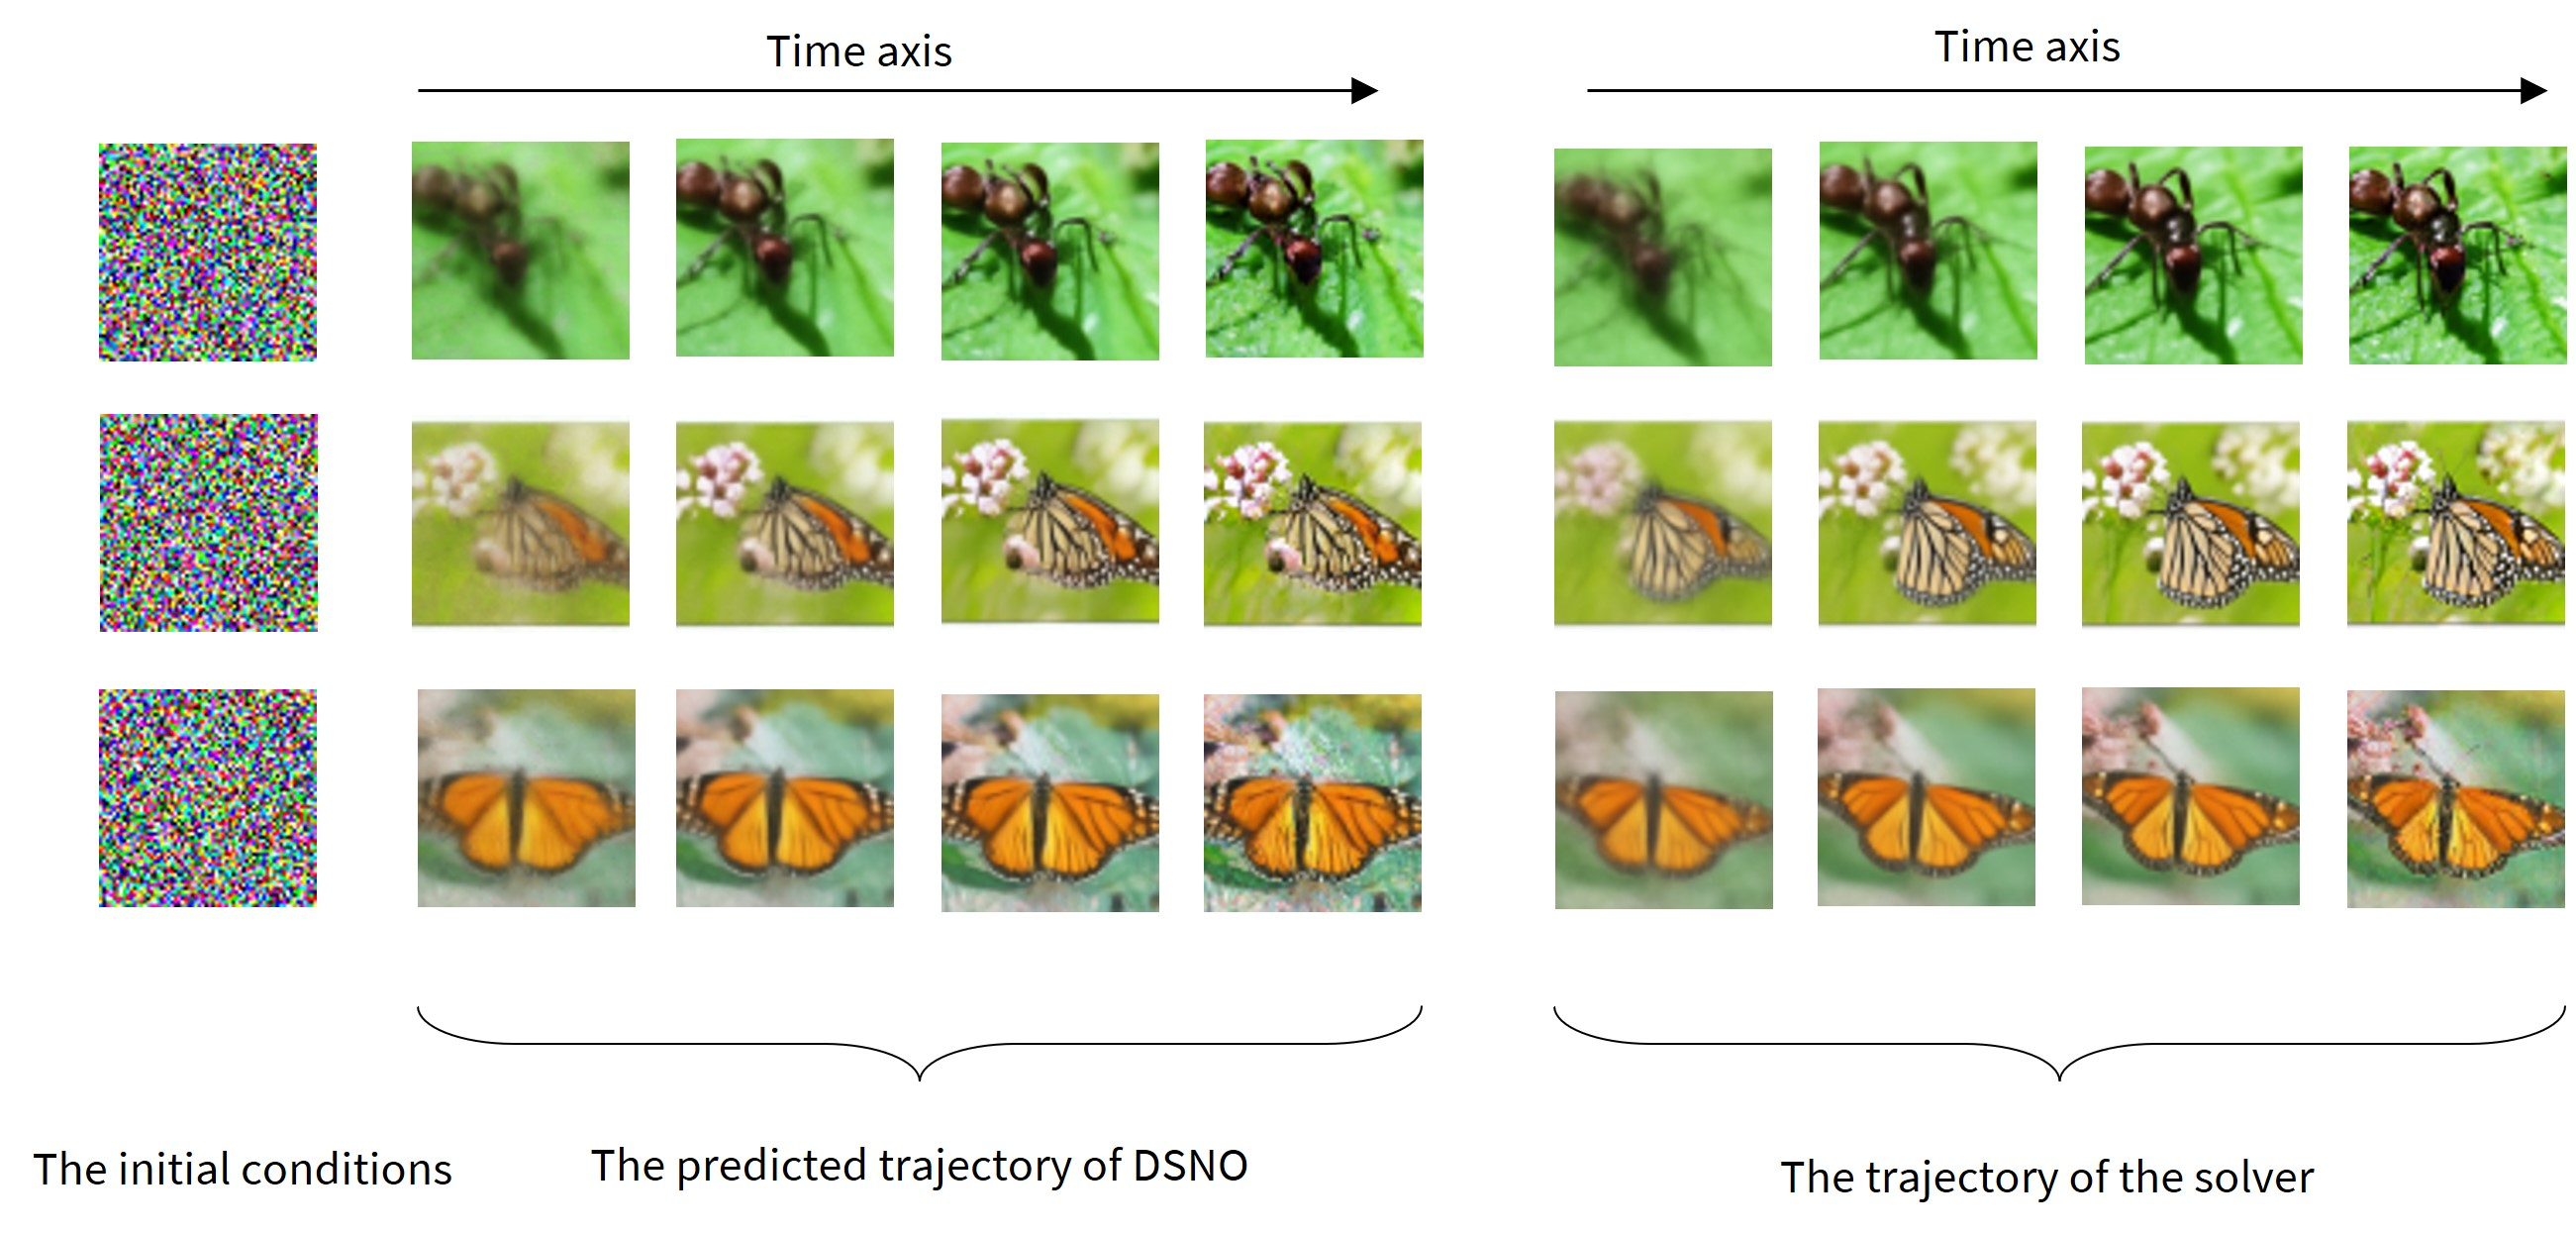
\includegraphics[width=0.97\columnwidth]{figs/demo_traj.jpg}
%         \caption{Comparison between the trajectory predicted by DSNO and the trajectory from the original solver on ImageNet-64, for the fixed random seed with a temporal resolution 4. Left: the prediction by DSNO. Right: the trajectory generated by solver. }
%         \label{fig:demo_imagenet_traj}
% \end{figure*}

\begin{figure}[t]
        \centering
        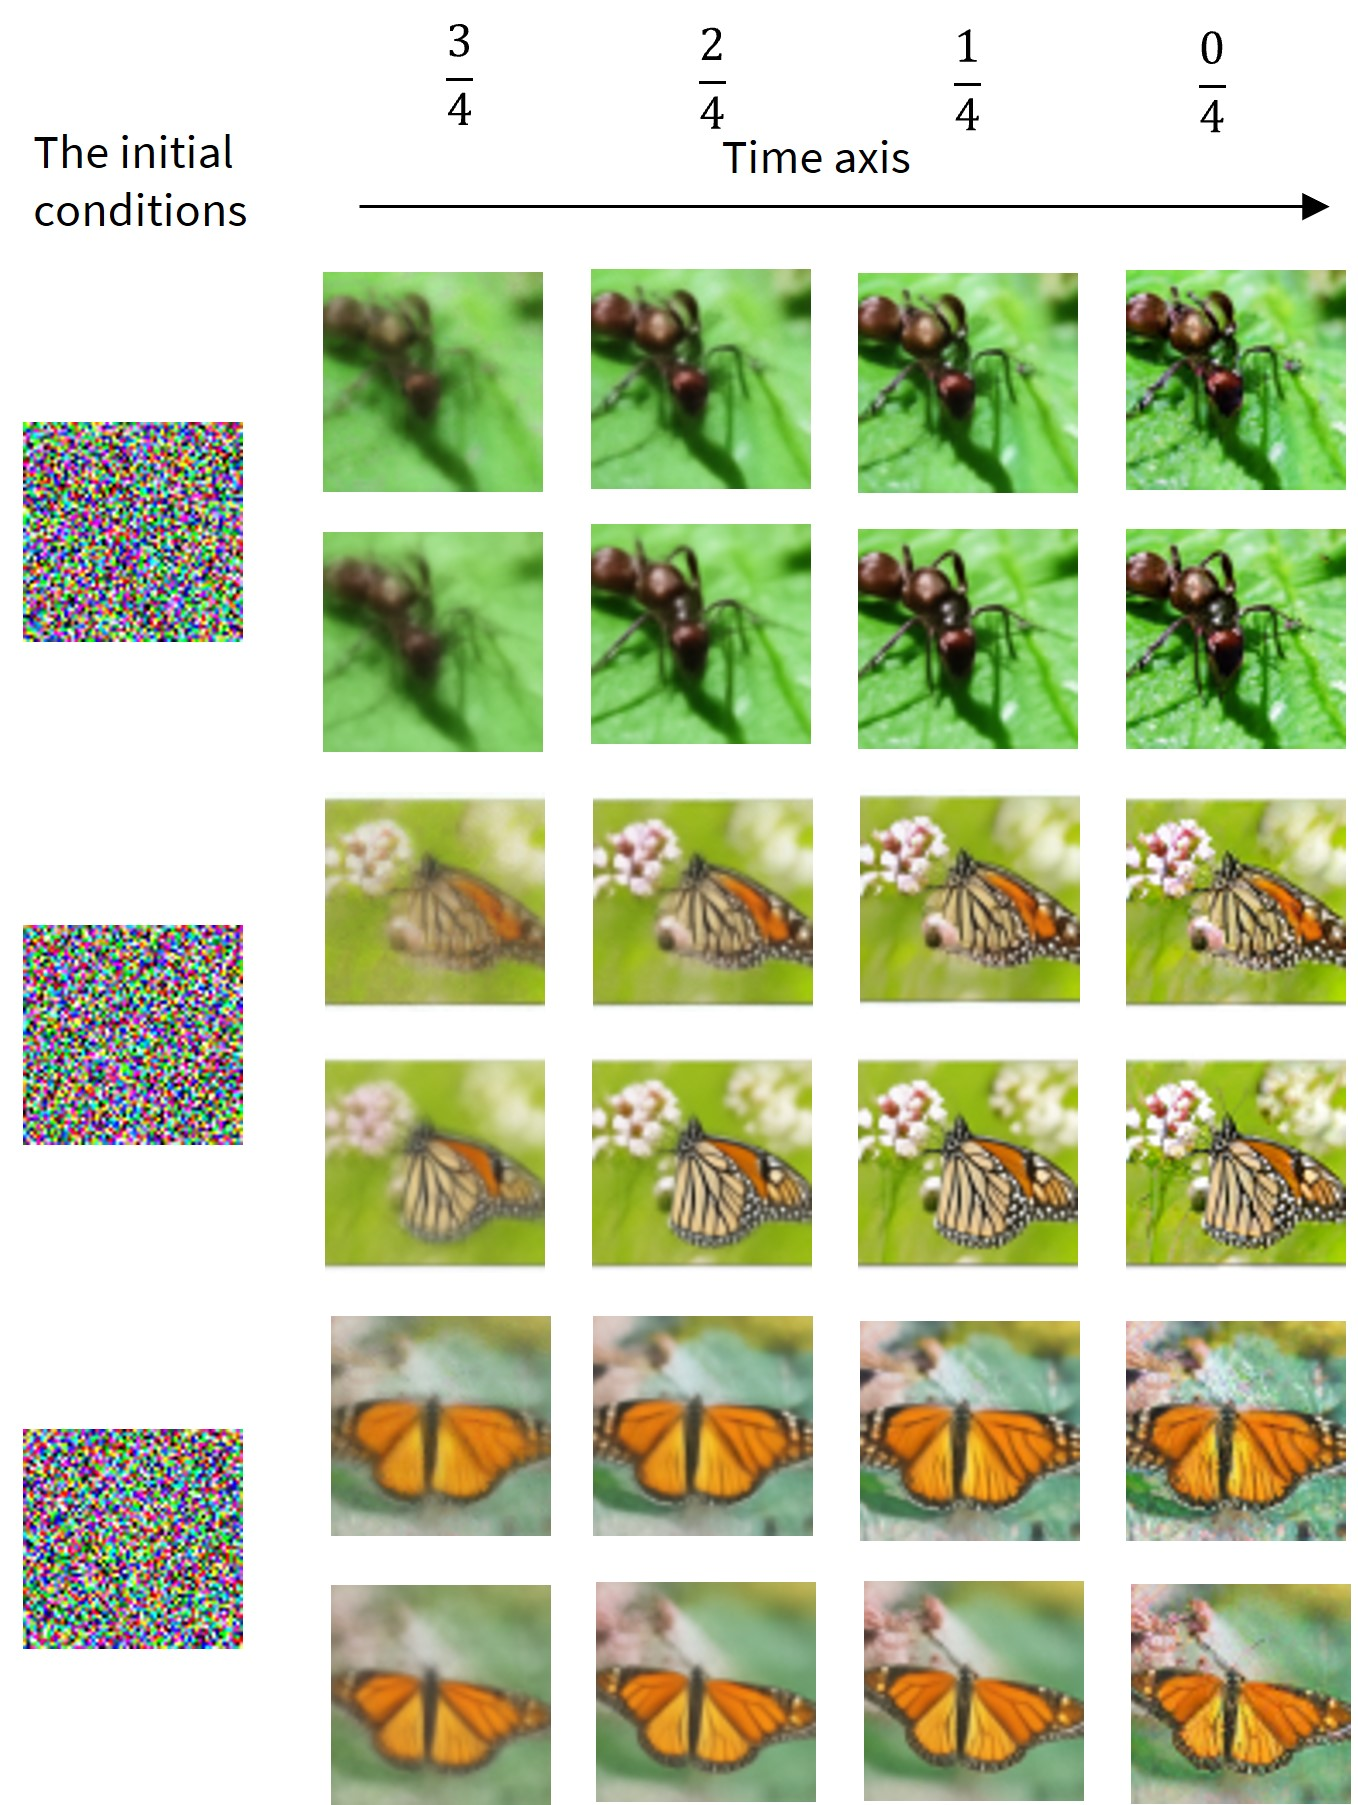
\includegraphics[width=0.97\columnwidth]{figs/demo_traj_1.jpg}
        \vspace{-3pt}
        \caption{Comparison between the trajectory predicted by DSNO and that from the original solver on ImageNet-64, for the fixed random seed with a temporal resolution 4. Upper row: the prediction by DSNO. Lower row: the trajectory generated by solver. }
        \label{fig:demo_imagenet_traj}
        \vspace{-5pt}
\end{figure}

% \begin{figure*}[ht]
%         \centering
%         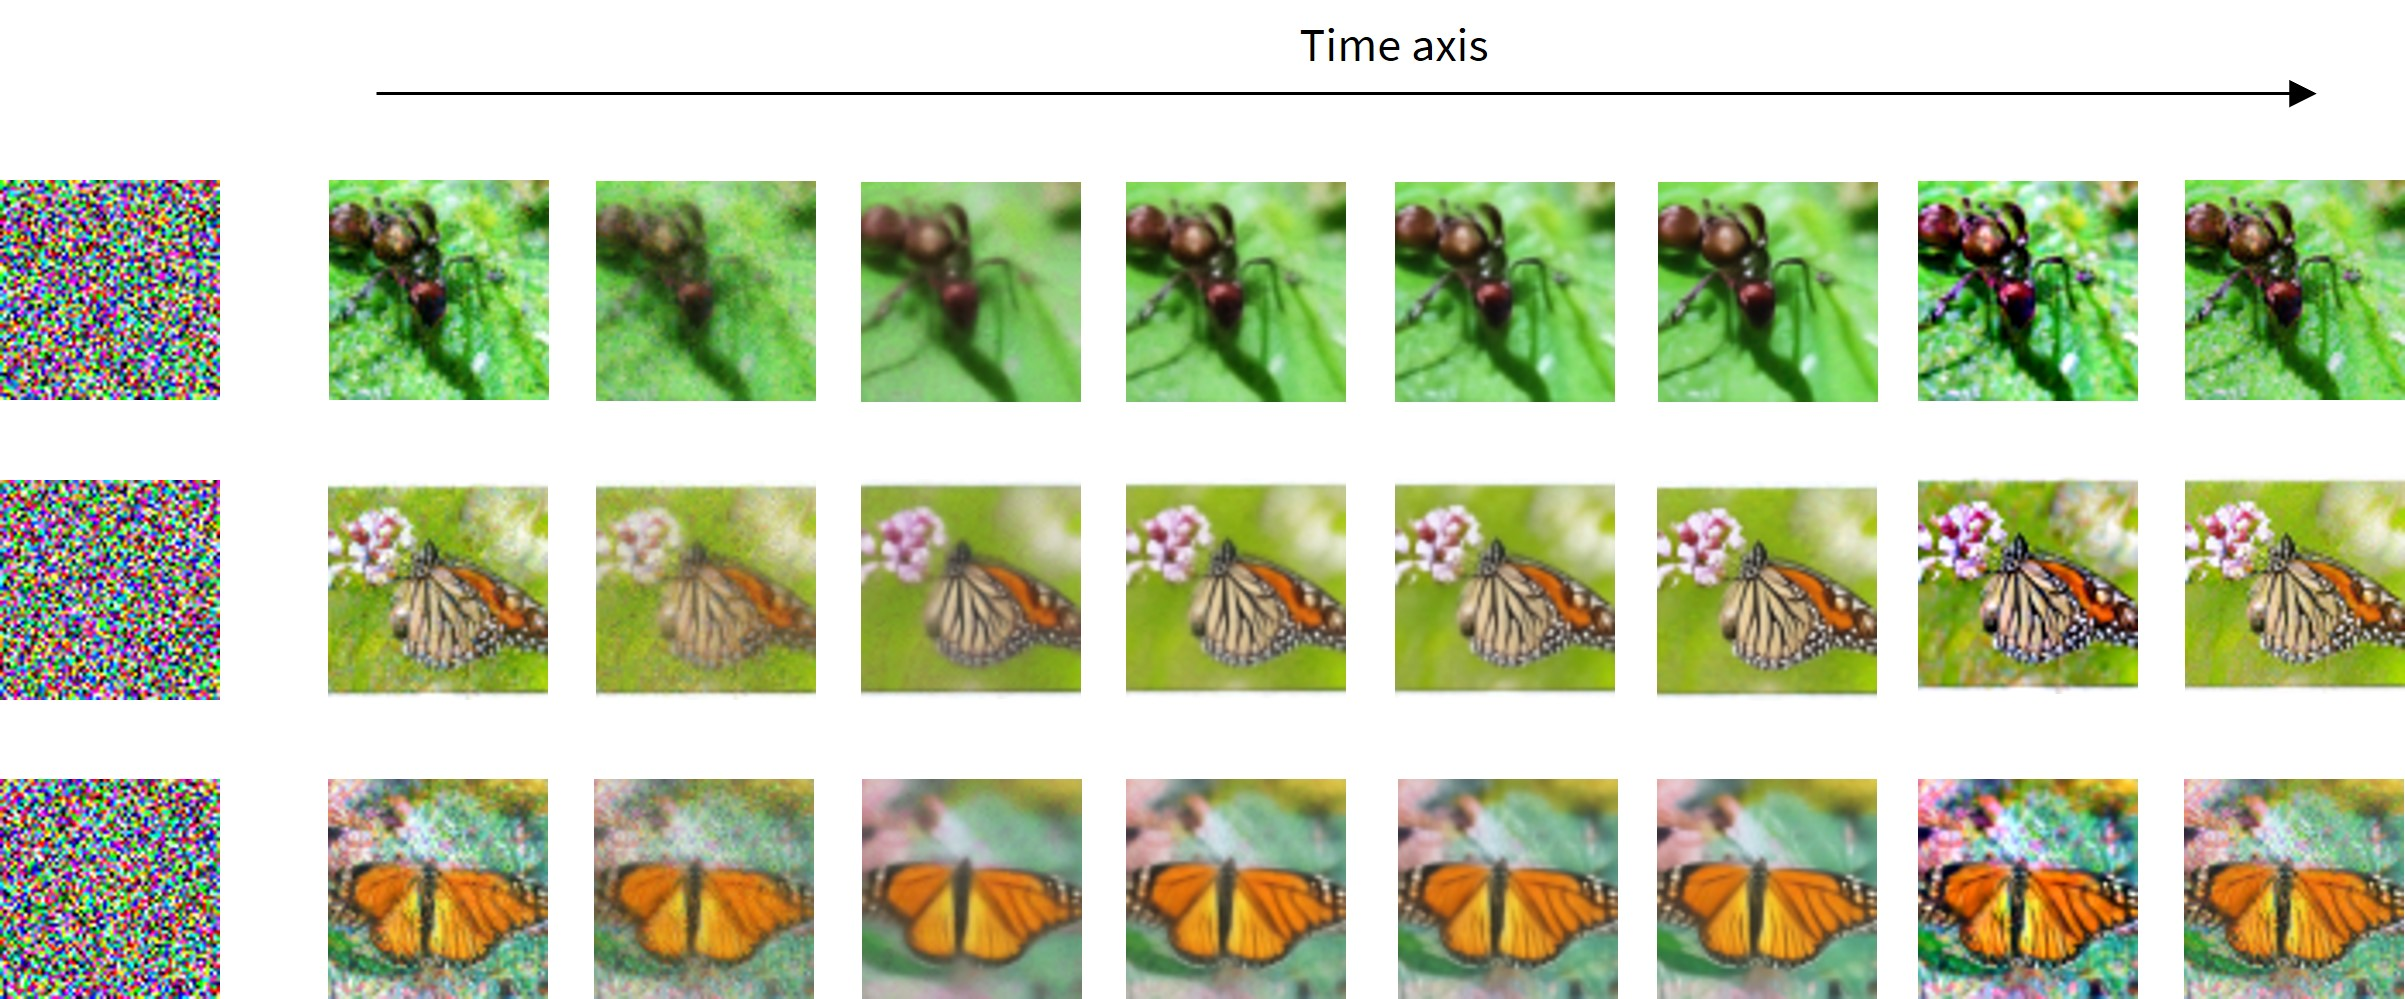
\includegraphics[width=0.75\textwidth]{figs/demo-high-res.jpg}
%         \caption{The predicted trajectory of DSNO in temporal resolution 8 on ImageNet-64. We train the DSNO with temporal resolution 4 and then use it to predict the trajectory with temporal resolution 8. }
%         \label{fig:demo_imagenet}
% \end{figure*}
\subsection{Conditional generation: ImageNet-64}
\paragraph{Trajectory data collection.} We generate 2.3 million trajectories with 16-step progressive distillation \cite{salimans2021progressive} using the pre-trained diffusion model from its official code base. The FID score of the generated training set is 2.70, computed over the first 50k training data points. 
\vspace{-0.1in}
\paragraph{Sampling quality and speed.} Table~\ref{tb:fid_imagenet} compares DSNO trained with a temporal resolution of 4 against the recent advanced fast sampling methods for diffusion models. 
DSNO clearly outperforms 1-step progressive distillation model and archives comparable FID  2-step models of progressive distillation with only one model evaluation. From Table~\ref{tb:speed_cifar}, DSNO has 1.7 times speedup over progressive distillation. The recall of DSNO is comparable to ADM's, showing that DSNO inherits the original diffusion model's diversity/mode coverage as it learns to solve the probability flow ODE. 

% \vspace{-0.1in}
% \paragraph{Model size and training cost.} The original architecture of the diffusion model contains 295,900,035 parameters. DSNO contains 329,225,091 parameters, which increases by around 10\% in model size. Training on ImageNet-64 takes about 7 days on 64 V100 GPUs with mixed precision. 

\vspace{-0.1in}
\paragraph{Trajectory prediction and reconstruction.}
Figure~\ref{fig:demo_imagenet_traj} compares the trajectories predicted by DSNO and the original ODE solver, respectively, for the fixed random seed with a temporal resolution 4. We see that the DSNO predicted trajectory highly matches the groundth-truth ODE trajectory, which demonstrates the effectiveness of DSNO with parallel decoding. Besides, Figure~\ref{fig:demo_imagenet_recon} shows the random samples from DSNO and the original pre-trained diffusion model with the same random seed. It is clear that the mapping from Gaussian noise to the output image is well-preserved.


\begin{figure}[ht]
        \centering
        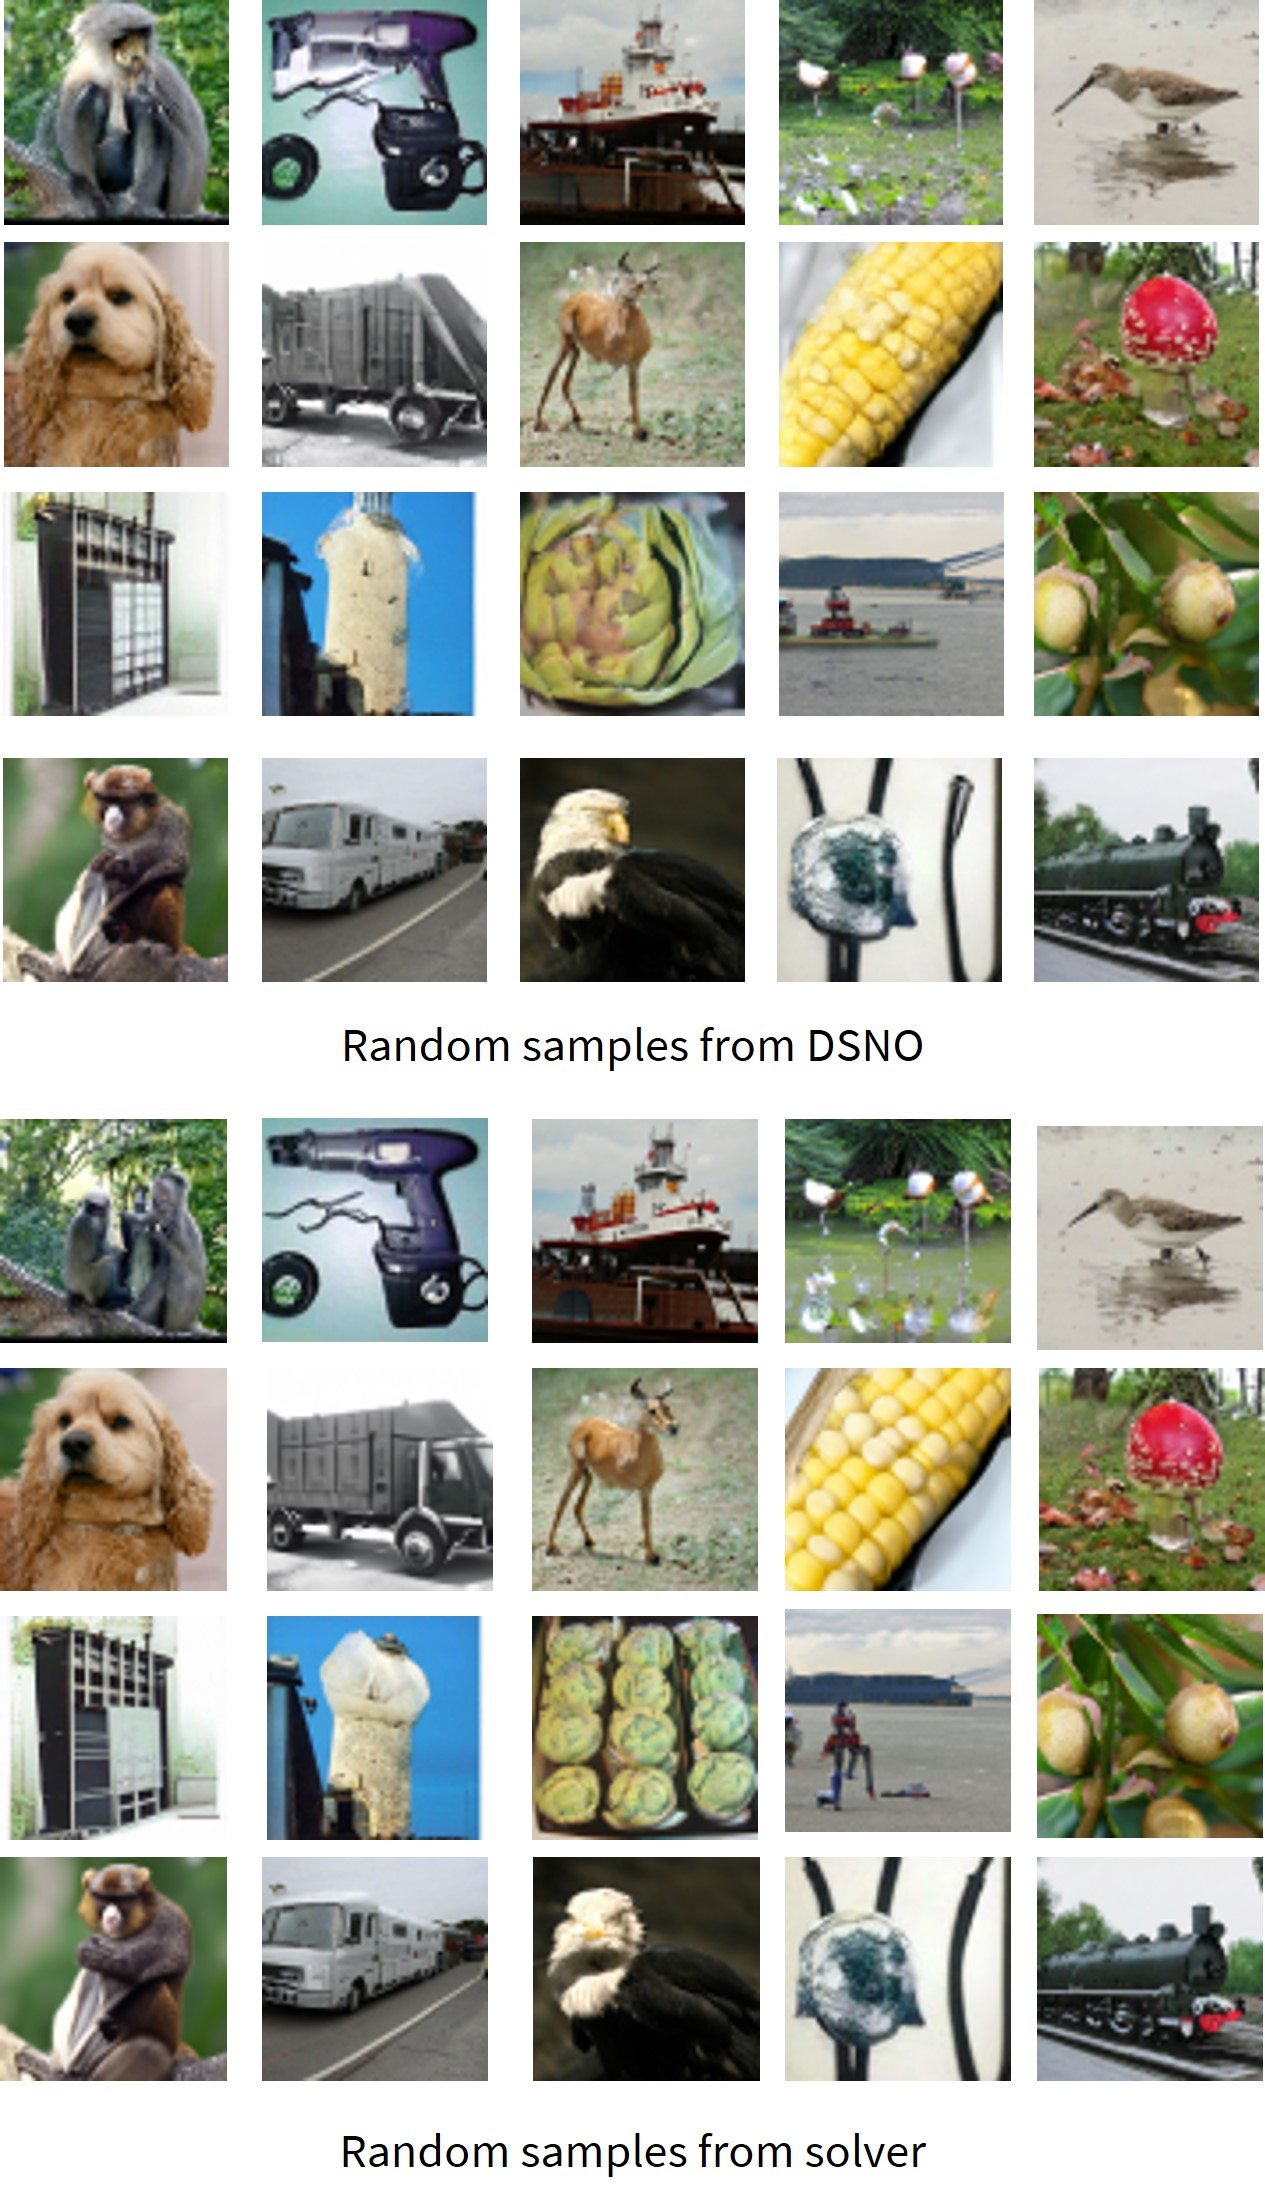
\includegraphics[width=0.8\columnwidth]{figs/demo_images.jpg}
        \caption{Upper panel: random samples generated by DSNO. Bottom panel: generated by the solver. }
        \label{fig:demo_imagenet_recon}
\end{figure}



\begin{table}[ht]
\caption{Impact of temporal convolution. We compare the performance of architectures with and without temporal convolution blocks while keeping all other settings the same. }
\label{tb:cifar_ablation_temporal_conv}
\begin{center}
\begin{small}
\begin{tabular}{lccc}
\toprule
 Training steps & U-Net &  U-Net + Temporal Conv \\
\midrule
300k  & 8.09 & 4.23 \\
400k & 7.85 & 4.12 \\ 
\bottomrule
\end{tabular}
\end{small}
\end{center}
\vskip -0.1in
\end{table}

\begin{table}[ht]
\caption{Ablation study on the choice of training loss weighting and time discretization scheme. The temporal resolution is fixed to 4 in this group of experiments. }
\label{tb:cifar_ablation_loss-weight}
\begin{center}
\begin{small}
\begin{tabular}{lcc}
\toprule
 Loss weighting & Uniform & $\mathrm{SNR}^{0.5}$ \\
% \midrule
FID  & 4.56 & 4.21 \\
\midrule
time discretization scheme & Uniform & Quadratic \\
% \midrule
FID & 4.33 & 4.21 \\
\bottomrule
\end{tabular}
\end{small}
\end{center}
\vskip -0.1in
\end{table}

\begin{table}[ht]
\caption{Ablation study on the choice of the temporal resolution.}
\label{tb:cifar_ablation_resolution}
\begin{center}
\begin{small}
\begin{tabular}{lccc}
\toprule
Temporal resolution & 2 & 4 & 8 \\
\midrule
FID  & 5.01 & 4.21  & 3.98\\
\bottomrule
\end{tabular}
\end{small}
\end{center}
\vskip -0.1in
\end{table}

\subsection{Ablation study}
In this section, we study the effect of different model choices, including the temporal convolution blocks, loss weighting function, temporal resolution, time discretization scheme, and loss function, by performing ablation studies on CIFAR-10. Without stated explicitly, we use batch size 128 and $\ell^1$ norm for the loss function. 
\vspace{-0.1in}
\paragraph{Temporal convolution block.} We first investigate the impact of temporal convolution by comparing the performance of architectures with and without temporal convolution blocks. All the other settings are kept the same such as temporal resolution 4, quadratic time discretization scheme, the square root of the SNR weighting function, and batch size 256. As reported in Table~\ref{tb:cifar_ablation_temporal_conv}, the temporal convolution design is crucial to DSNO's performance as its kernel integration operator nature is a better model inductive bias to model the trajectory in time. 



\vspace{-0.1in}
\paragraph{Loss weighting.}  The loss weighting function used in the training objective of Diffusion models\cite{ho2020denoising, song2020score} typically distributes more weights to the small times, which is important to training diffusion models. We also adopt such a weighting function since it is generally harder to control the error at small times. We observe that such loss weighting function benefits the training of DSNO. As reported in Table~\ref{tb:cifar_ablation_loss-weight}, using the square root of the SNR weighting function slightly improves the FID by 0.35. 
\vspace{-0.1in}
\paragraph{Time discretization scheme.} How to discretize the temporal domain is important to the performance of the numerical solvers. Some small changes to the time discretization scheme could lead to very different sample qualities as shown in~\cite{karras2022elucidating,zhang2022fast}. DSNO also needs to choose a way to discretize the temporal domain. Here we consider the two most common choices of time discretization schemes in the literature: uniform time step and quadratic time step. As shown in Table~\ref{tb:cifar_ablation_loss-weight}, the quadratic time step is slightly better than the uniform time step by 0.12, showing that DSNO is not sensitive to the different time discretization schemes used in the existing solvers and can work nicely with different solvers. 
\vspace{-0.1in}
\paragraph{Temporal resolution.} We study the effect of temporal resolution (i.e., the discretization steps $M$), given the square root of SNR weighting function and the quadratic time discretization scheme. 
% We train different models with temporal resolutions ranging from 2 to 8 with the model parameter $J$ set to half of the resolution. 
As reported in Table~\ref{tb:cifar_ablation_resolution}, the FID improves as we increase the temporal resolution. Since the higher temporal resolution introduces more supervision into the training, it is reasonable to expect better FID scores. However, higher resolution also results in higher computation costs. Since increasing the resolution from 4 to 8 only provides a marginal benefit (due to the compact spectrum we observed in Appendix~\ref{sec:spectrum}), one may use temporal resolution 4 for better efficiency.   

\begin{table}[ht]
\caption{Ablation study on the choice of the loss function. For LPIPS, we use the original VGG-based version without any calibration~\cite{zhang2018unreasonable}.}
\label{tb:cifar_ablation_loss}
\begin{center}
\begin{small}
\begin{tabular}{lcc}
\toprule
Loss function & $\ell^1$ & LPIPS \\
\midrule
FID   & 4.12  & 3.78 \\
\bottomrule
\end{tabular}
\end{small}
\end{center}
\vskip -0.1in
\end{table}
\paragraph{Loss function.} We only vary the loss function but keep the other settings the same, including a batch size of 256, a temporal resolution of 4, and a quadratic discretization scheme.  As shown in Table~\ref{tb:cifar_ablation_loss}, using the original VGG-based LPIPS loss~\cite{zhang2018unreasonable} instead of the standard $\ell^1$ loss leads to a further improvement in the FID score. 
% Table~\ref{tb:cifar_ablation_loss-weight} reports the results of our ablation study. We observe that higher resolution provides stronger supervision and improves the sample quality. Further increasing resolution from 4 to 8 obtains marginal benefit. The quadratic time discretization scheme and $1/\sigma_t$ loss weighting are two common heuristics used in diffusion models. Our experiments show using the same time discretization scheme and loss weighting as used in diffusion model training improves the sample quality. 

% \begin{figure}[ht]
%         \centering
%         \includegraphics[width=0.8\columnwidth]{figs/cifar_ablation_tr.pdf}
%         \caption{FID score of generated samples versus the temporal resolution of the model. }
%         \label{fig:cifar_ablation}
% \end{figure}





\section{Related work}

\paragraph{ODE-based sampling.}
ODE-based samplers are much more widely used in practice \cite{stablediffusion} than SDE-based methods because they can take large time steps by leveraging some useful structures of the underlying ODE such as semi-linear structure and the form of exponentially weighted integral \cite{lu2022dpm, zhang2022fast}. Existing works \cite{song2021denoising, bao2021analytic, zhang2022fast,dockhorn2022genie} have greatly reduced the number of discretization steps to 10-50 in time while keeping the approximation error small to generate high-quality samples. The exponentially weighted integral structure of the solution trajectory revealed by prior works also inspired our design of the temporal convolution block. 
% We note that these advanced numerical solvers allow us to approximate the solution operator with less computation cost, which greatly speeds up our training data generation process and also benefits other training-based methods.  
 % In this paper, we also use some of the advanced ODE-based solvers to generate our training set for DSNO. 
\vspace{-0.1in}
\paragraph{Operator learning for solving PDEs.}
Neural operators are deep learning models that are designed for mappings between function spaces, i.e., continuous functions~\cite{li2020neural,kovachki2021universal}. They are widely deployed as the de facto deep learning models in scientific computing when dealing with partial differential equations (PDE).
% Operator learning is a successful learning paradigm in the scientific computing area for solving partial differential equations. It contains a diverse class of methods including DeepOnet-based methods and neural operator methods including \citet{li2020neural, li2020multipole, li2020fourier}. 
Among these methods, Fourier neural operator stands out and is one of the most efficient machine learning methods for scientific computing problems involving PDE
\cite{yang2021seismic,wen2022accelerating}. It is shown to possess the crucial discretization invariance and universal approximation properties of universal operators~\citep{kovachki2021universal,kovachki2021neural}, which motivates our design of the temporal convolution block in our method.


\vspace{-0.1in}
\paragraph{Training-based sampling.} Training-based methods typically train a neural network surrogate to replace some parts of the numerical solver or even the whole solver. This category includes various methods from diverse perspectives such as knowledge distillation \cite{luhman2021knowledge, salimans2021progressive}, learning the noise schedule \cite{lam2021bilateral, watson2021learning}, learning the reverse covariance \cite{bao2022estimating}, which require extra training. Training-based methods usually work in the few-step regime with less than 10 steps. Direct \citet{luhman2021knowledge} is the first work to get descent sample quality on CIFAR10 with one model evaluation but it suffers from overfitting and its sampling quality drops dramatically compared to the original sampling methods of diffusion models. The current SOTA progressive distillation \cite{salimans2021progressive} reduces the number of steps down to 4-8 without losing much sample quality. However, it has the same issue as knowledge distillation in the limit of one function evaluation. Some other methods~\cite{xiao2021tackling,vahdat2021score, zheng2022truncated} combine diffusion models with other generative models such as GAN and VAE to enable fast sampling. 
% For example, DDGAN \cite{xiao2021tackling} achieves excellent FID scores with as few as 4 steps by leveraging conditional GAN to model the denoising distributions or equivalently the reverse stochastic process, allowing for large denoising steps. But it involves adversarial training like GAN does which can be potentially harder to train than the methods that directly utilize the pre-trained diffusion models. LSGM \cite{vahdat2021score} greatly accelerates sampling by learning an encoder that transforms the data distribution into a smooth latent distribution that is close to a Gaussian prior so that the reverse process is smooth and allows for large time steps. LSGM requires 20 to 100 steps to generate reasonable samples. 
% \paragraph{Parallel decoding.} Parallel decoding is mainly used for the discrete tokens in the language models~\cite{ghazvininejad2019mask} and vision transformers~\cite{chang2023muse}, which can predict multiple tokens with only one model forward pass. 



\section{Conclusion and discussion}
In this paper, we propose \textit{diffusion model sampling with neural operator} (DSNO) that maps the initial condition, i.e., Gaussian distribution, to the continuous-time solution trajectory of the reverse diffusion process. To better model the temporal correlations along the trajectory, we introduce temporal convolution layers into the given diffusion model backbone.  Experiments show that our method achieves the SOTA FID score of 3.78 for CIFAR-10 and 7.83 for ImageNet-64 with only one model evaluation. 
Our method is a big step toward real-time sampling of diffusion models, which can potentially benefit many time-sensitive applications of diffusion models. 


\section*{Acknowledgements}
We would like to thank the reviewers and the area chair for their constructive comments. Anima Anandkumar is supported in part by Bren professorship. This work was done partly during Hongkai Zheng's internship at NVIDIA.
% Note use of \abovespace and \belowspace to get reasonable spacing
% above and below tabular lines.

% Acknowledgements should only appear in the accepted version.


% \textbf{Do not} include acknowledgements in the initial version of
% the paper submitted for blind review.

% If a paper is accepted, the final camera-ready version can (and
% probably should) include acknowledgements. In this case, please
% place such acknowledgements in an unnumbered section at the
% end of the paper. Typically, this will include thanks to reviewers
% who gave useful comments, to colleagues who contributed to the ideas,
% and to funding agencies and corporate sponsors that provided financial
% support.


% In the unusual situation where you want a paper to appear in the
% references without citing it in the main text, use \nocite
\nocite{langley00}

\bibliography{icml_ref}
\bibliographystyle{icml2023}


%%%%%%%%%%%%%%%%%%%%%%%%%%%%%%%%%%%%%%%%%%%%%%%%%%%%%%%%%%%%%%%%%%%%%%%%%%%%%%%
%%%%%%%%%%%%%%%%%%%%%%%%%%%%%%%%%%%%%%%%%%%%%%%%%%%%%%%%%%%%%%%%%%%%%%%%%%%%%%%
% APPENDIX
%%%%%%%%%%%%%%%%%%%%%%%%%%%%%%%%%%%%%%%%%%%%%%%%%%%%%%%%%%%%%%%%%%%%%%%%%%%%%%%
%%%%%%%%%%%%%%%%%%%%%%%%%%%%%%%%%%%%%%%%%%%%%%%%%%%%%%%%%%%%%%%%%%%%%%%%%%%%%%%
\newpage
\appendix
\onecolumn

\section{Appendix}

\subsection{Energy spectrum}
\label{sec:spectrum}
The discrete-time Fourier transform of the signal $x(t)$ with period $T$ is given by 
\begin{equation}
    X_j = \sum_{i=1}^{N} x(t_i) \exp\left(-\frac{2\pi}{T} ji t_i\right), 
\end{equation}
where $t_i = \frac{iT}{N}$. $\frac{j}{T}$ is the frequency. $j$ is called the frequency mode. Let $\Delta = \frac{1}{N}$ be the time step. The spectrum is defined as the product of the Fourier transform of $x$ with its conjugate:
\begin{equation}
    S_{j} = \frac{2\Delta^2}{T} X_j X_j^{*},
\end{equation}
where $X_j^{*}$ is the complex conjugate. In practice, the statistics are computed over all pixel locations and channels of randomly generated trajectories. $T=1$ and the sampling frequency is 1000 Hz to avoid aliasing. Figure~\ref{fig:spectrum} visualizes the energy spectrum of ODE trajectories sampled from the diffusion model "DDPM++ cont. (VP)" trained by \cite{song2020score} on CIFAR10. We observe that most power concentrates in the regime where the frequency mode is less than 5. 

\begin{figure}[htbp]
    \centering
    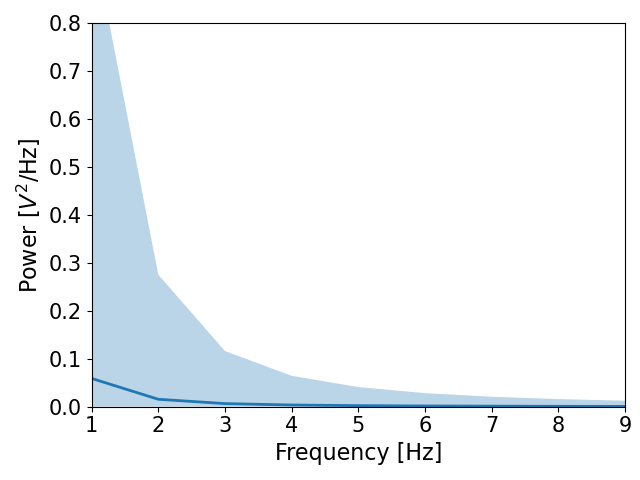
\includegraphics[width=0.5\columnwidth]{figs/power_spectrum.png}
    \caption{Power spectrum of the ODE trajectories sampled from "DDPM++ cont. (VP)" model trained by \cite{song2020score} on CIFAR10. The mean is computed over all pixel locations and channels of randomly generated trajectories. Most power concentrates in the $\leq 5$ Hz regime. The shaded region represents the maximum and minimum power.  }
    \label{fig:spectrum}
    % \caption{Compact spectrum and DFNO architecture design.}
\end{figure}

\subsection{Background: neural operators}
\label{sec:neural_operator}
Let $\mathcal{A}$ and $\mathcal{U}$ be two Banach spaces and $G: \mathcal{A} \rightarrow \mathcal{U}$ be a non-linear map. 
Suppose we have a finite collection of data $\{a_i, u_i\}_{i=1}^{N}$ where $a_i\sim \mu$ are i.i.d. samples from the distribution $\mu$ supported on $\mathcal{A}$ and $u_i=G(a_i)$.
Neural operators aim to learn $G_{\phi}$ parameterized by $\phi$ to approximate $G$ from the observed data by minimizing the empirical risk given by
\begin{equation}
    \min_{\phi} \mathbb{E}_{a\sim \mu} \|G(a) - G_{\phi}(a)\|_{\mathcal{U}} \approx \min_{\phi} \frac{1}{N} \sum_{i=1}^{N} \|u_i - G_{\phi}(a_i)\|_\mathcal{U}.
\end{equation}


The architecture of neural operators is constructed as a stack of kernel integration layers where the kernel function is parameterized by learnable weights. This architecture utilizes the convolution theorem on abelian groups. Among different neural operator architectures, Fourier neural operator~\cite{li2020fourier} stands out and is one of the most efficient machine learning methods for scientific computing problems involving PDE
\cite{yang2021seismic,wen2022accelerating}. It is shown to possess the crucial discretization invariance and universal approximation properties of universal operators~\citep{kovachki2021universal,kovachki2021neural}.


\subsection{Extended set of generated samples}
We provide an extended set of randomly generated samples from our ImageNet-64 model in Figure~\ref{fig:images_set1}. 
\begin{figure}[htbp]
    \centering
    \includegraphics[width=0.6\textwidth]{figs/dsno-set1-min.pdf}
    \caption{Random samples generated from DSNO on ImageNet-64.}
    \label{fig:images_set1}
\end{figure}




\subsection{Generalization to different resolution}

Figure~\ref{app_fig:demo_imagenet} visualizes the predicted trajectory of DSNO in temporal resolution 8 on ImageNet-64 while it is trained on temporal resolution 4. Although the resulting trajectories do not look perfectly smooth, it still demonstrates the generalization ability of DSNO to unseen time resolutions.



% \subsection{Related work}
% \paragraph{ODE-based sampling.}
% ODE-based samplers are much more widely used in practice \cite{stablediffusion} than SDE-based methods because they can take large time steps by leveraging some useful structures of the underlying ODE such as semi-linear structure and the form of exponentially weighted integral \cite{lu2022dpm, zhang2022fast}. Existing works \cite{song2021denoising, bao2021analytic, zhang2022fast,dockhorn2022genie} have greatly reduced the number of discretization steps to 10-50 in time while keeping the approximation error small to generate high-quality samples. The exponentially weighted integral structure of the solution trajectory revealed by prior works also inspired our design of the temporal convolution block. We note that these advanced numerical solvers allow us to approximate the solution operator with less computation cost, which greatly speeds up our training data generation process and also benefits other training-based methods.  
%  % In this paper, we also use some of the advanced ODE-based solvers to generate our training set for DSNO. 

% \paragraph{Operator learning for solving PDEs.}
% Neural operators are deep learning models that are designed for mappings between function spaces, i.e., continuous functions~\cite{li2020neural,kovachki2021universal}. They are widely deployed as the de facto deep learning models in scientific computing when dealing with partial differential equations (PDE).
% % Operator learning is a successful learning paradigm in the scientific computing area for solving partial differential equations. It contains a diverse class of methods including DeepOnet-based methods and neural operator methods including \citet{li2020neural, li2020multipole, li2020fourier}. 
% Among these methods, Fourier neural operator stands out and is one of the most efficient machine learning methods for scientific computing problems involving PDE
% \cite{yang2021seismic,wen2022accelerating}. 
% This architecture utilizes the convolution theorem on abelian groups and is shown to possess the crucial discretization invariance and universal approximation properties of universal operators~\citep{kovachki2021universal,kovachki2021neural}, which motivates our design of the temporal convolution block in our method.

% \paragraph{Training-based sampling.} Training-based methods typically train a neural network surrogate to replace some parts of the numerical solver or even the whole solver. This category includes various methods from diverse perspectives such as knowledge distillation \cite{luhman2021knowledge, salimans2021progressive}, learning the noise schedule \cite{lam2021bilateral, watson2021learning}, learning the reverse covariance \cite{bao2022estimating}, which require extra training. Training-based methods usually work in the few-step regime with less than 10 steps. Direct \citet{luhman2021knowledge} is the first work to get descent sample quality on CIFAR10 with one model evaluation but it suffers from overfitting and its sampling quality drops dramatically compared to the original numerical sampling methods in diffusion models. The current SOTA progressive distillation \cite{salimans2021progressive} reduces the number of steps down to 4-8 without losing much sample quality. However, it has the same issue as knowledge distillation in the limit of one function evaluation. Some other methods~\cite{xiao2021tackling,vahdat2021score} combine diffusion models with other generative models such as GAN and VAE to enable fast sampling. 

% \paragraph{Diffusion + GANs.} 

\subsection{Further discussion}
\paragraph{Future work}
There are several directions we leave as future work. First, guided sampling of diffusion models is widely used in various applications but accelerating guided sampling is also more challenging~\cite{meng2022distillation}. How to adapt DSNO for sampling Guided diffusion model will be an interesting next step. 
Second, the temporally continuous output of DSNO provides another level of flexibility compared to distillation-based methods and is readily available for applications such as DiffPure~\cite{nie2022DiffPure} that require fast forward/backward sampling from diffusion models at various temporal locations. DSNO could potentially reduce the inference time in those applications.
We leave the exploration of those applications to future work. Last but not least, transformer-based architectures have shown their promising capacity for diffusion models~\cite{peebles2022scalable, bao2023all} in high-resolution image generation. It is natural to integrate our temporal convolution layers into these diffusion transformers as the temporal blocks operate solely on the temporal dimension regardless of how the pixel space is modeled. The resulting new architecture could also potentially serve as a new architecture design for other problems where the dynamics are continuous in time. 

\paragraph{Reducing data collection cost with advanced solvers.} While we primarily use DDIM solver to collect data for fair comparison in this paper, it is worth noting that advanced numerical solvers like DPM solver\cite{lu2022dpm} can approximate the solution operator with less computation cost, which will greatly speed up our training data generation process. Our final implementation includes examples of using DPM solvers in our GitHub repository \href{https://github.com/devzhk/DSNO-pytorch}{https://github.com/devzhk/DSNO-pytorch}. 



\begin{figure*}[ht]
        \centering
        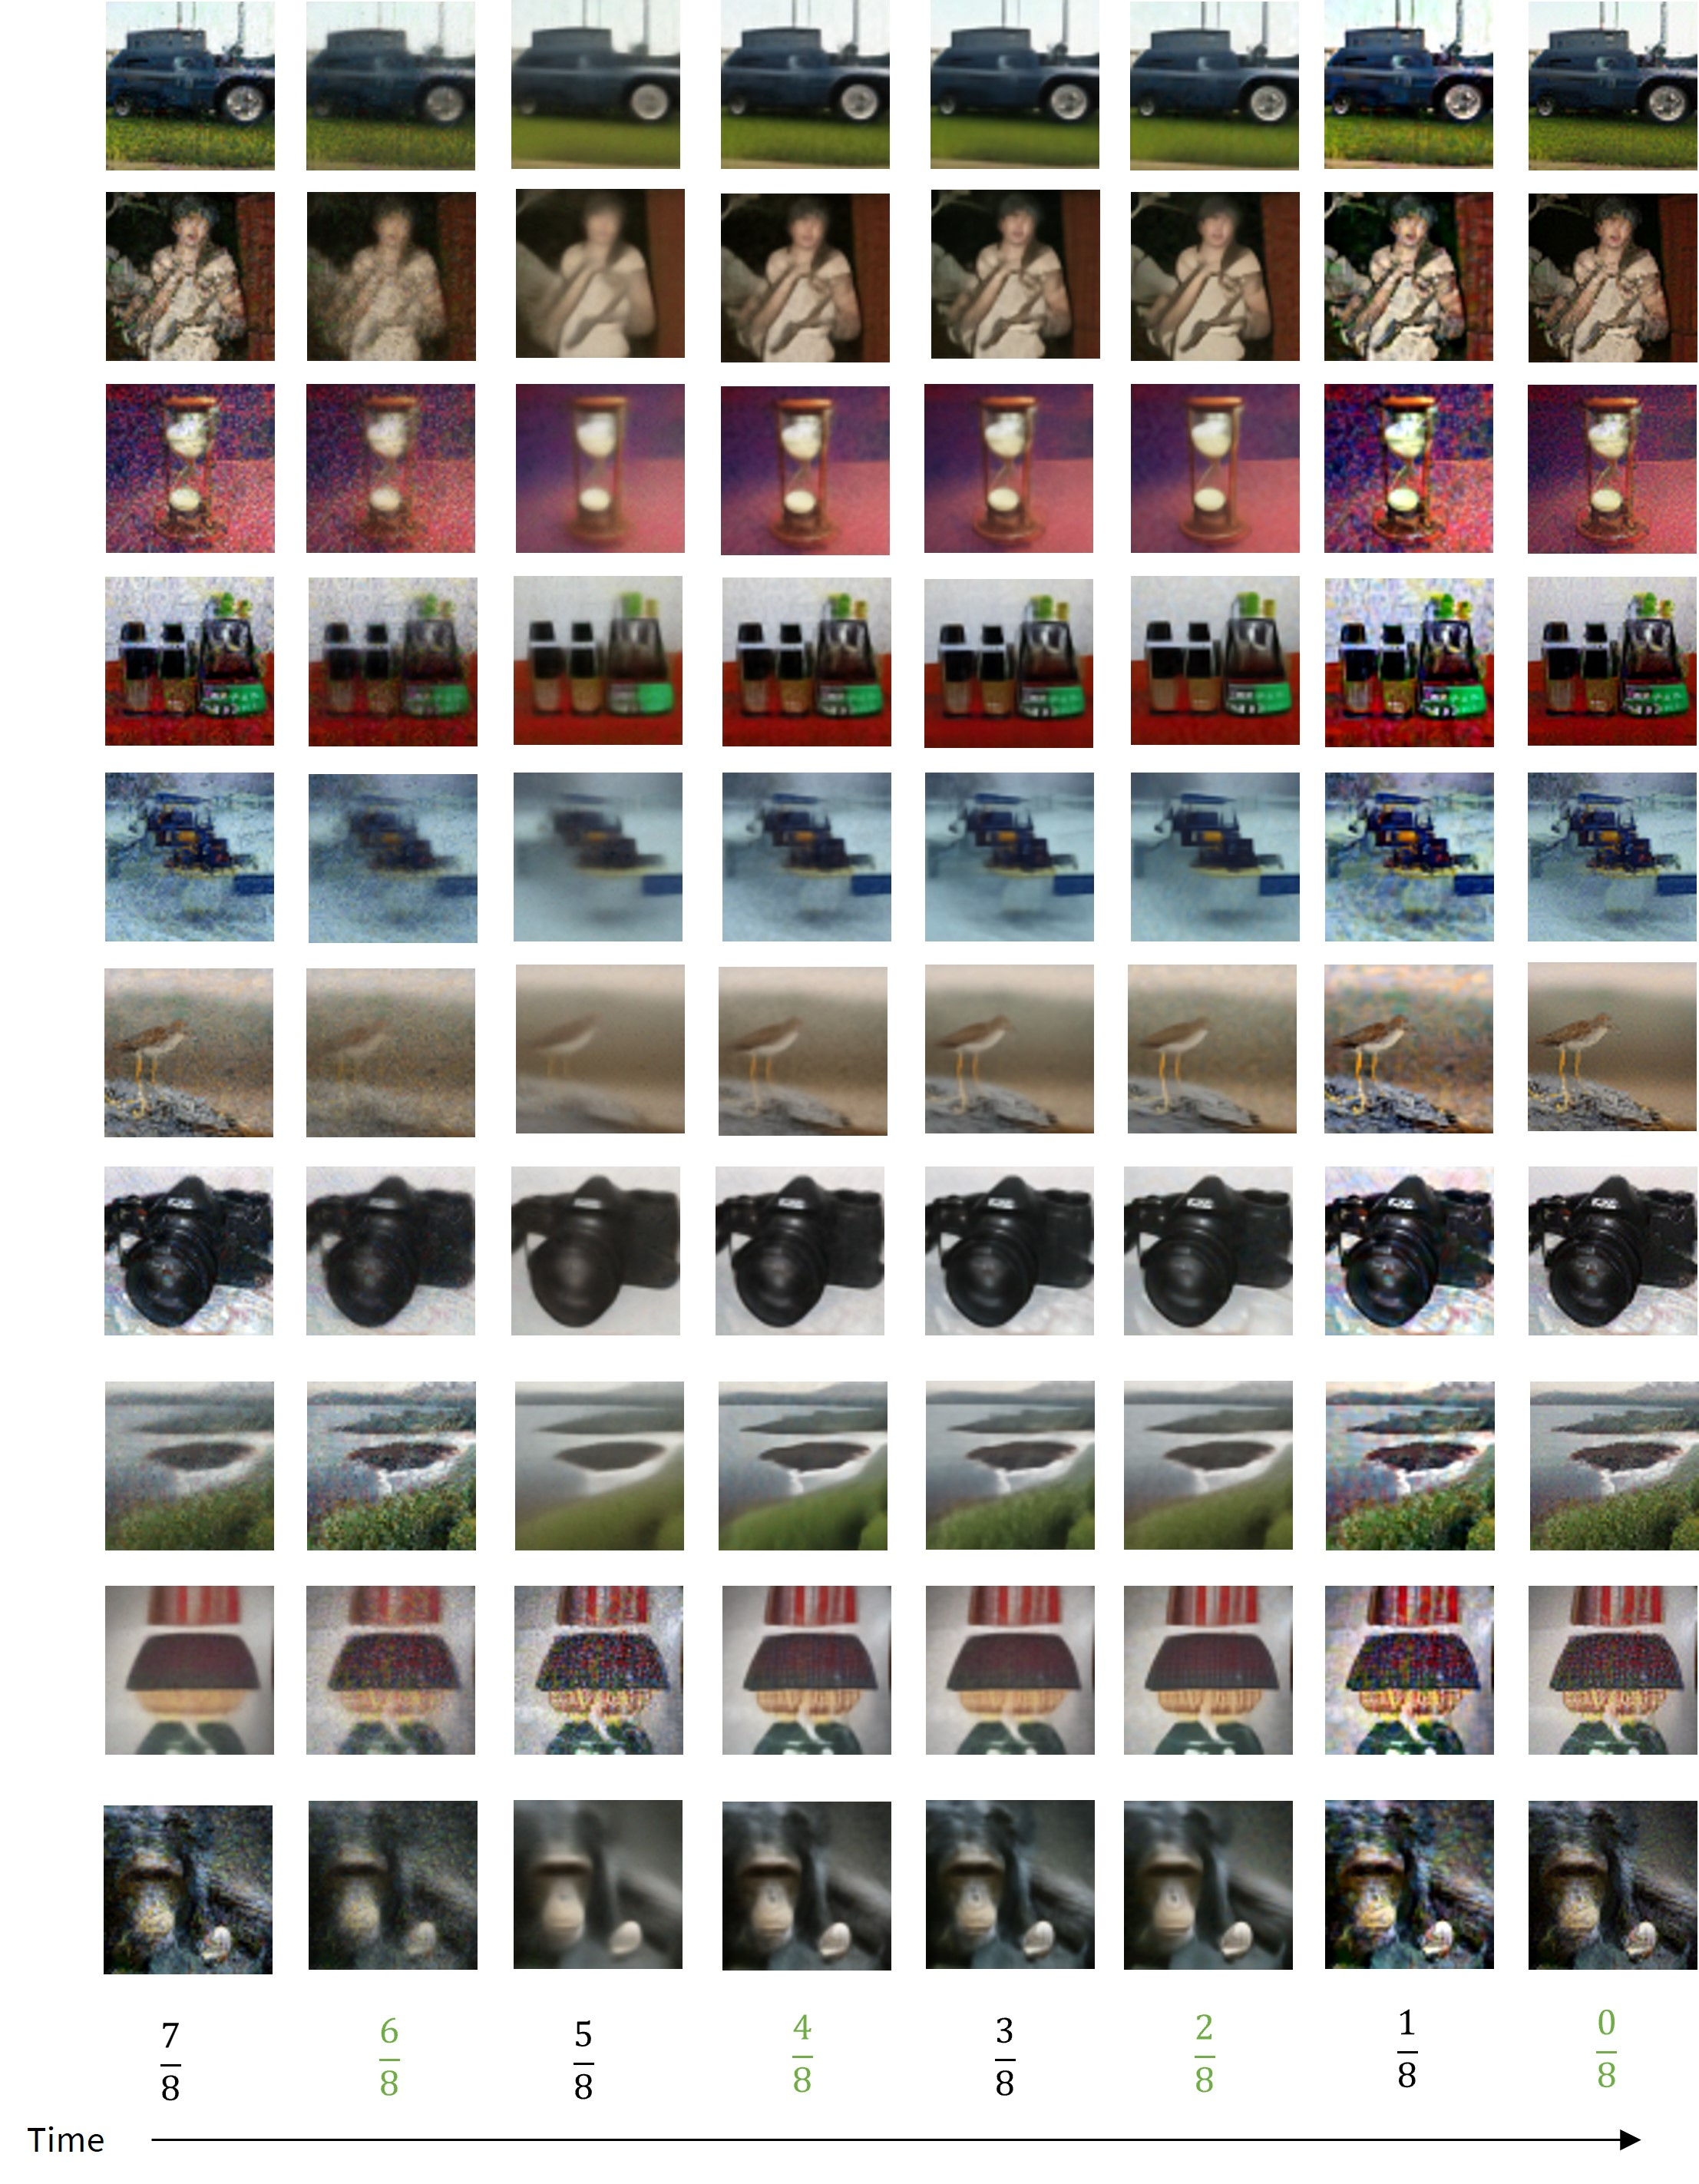
\includegraphics[width=0.75\textwidth]{figs/demo_high-res-app-1.jpg}
        \caption{The predicted trajectory of DSNO with a temporal resolution of 8 on ImageNet-64. We train the DSNO with a temporal resolution of 4 and then use it to predict the trajectory with a temporal resolution of 8. Time locations marked green are the points that DSNO is trained with. Black time locations are the points that DSNO never saw in the training set. }
        \label{app_fig:demo_imagenet}
\end{figure*}

%%%%%%%%%%%%%%%%%%%%%%%%%%%%%%%%%%%%%%%%%%%%%%%%%%%%%%%%%%%%%%%%%%%%%%%%%%%%%%%
%%%%%%%%%%%%%%%%%%%%%%%%%%%%%%%%%%%%%%%%%%%%%%%%%%%%%%%%%%%%%%%%%%%%%%%%%%%%%%%


\end{document}


% This document was modified from the file originally made available by
% Pat Langley and Andrea Danyluk for ICML-2K. This version was created
% by Iain Murray in 2018, and modified by Alexandre Bouchard in
% 2019 and 2021 and by Csaba Szepesvari, Gang Niu and Sivan Sabato in 2022.
% Modified again in 2023 by Sivan Sabato and Jonathan Scarlett.
% Previous contributors include Dan Roy, Lise Getoor and Tobias
% Scheffer, which was slightly modified from the 2010 version by
% Thorsten Joachims & Johannes Fuernkranz, slightly modified from the
% 2009 version by Kiri Wagstaff and Sam Roweis's 2008 version, which is
% slightly modified from Prasad Tadepalli's 2007 version which is a
% lightly changed version of the previous year's version by Andrew
% Moore, which was in turn edited from those of Kristian Kersting and
% Codrina Lauth. Alex Smola contributed to the algorithmic style files.
